% !TeX program = lualatex
% !TeX encoding = utf8
% !TeX spellcheck = uk_UA
% !BIB program = bibler

\documentclass{beamer}
\usetheme{Electromagnetism}
\usepackage{Electromagnetism}
\hypersetup{
  colorlinks=true,
  linkcolor=cyan,  % Цвет для внутренних ссылок
  urlcolor=red,    % Цвет для URL
  citecolor=blue   % Цвет для библиографических ссылок
}




%============================================================================
\title[Лекції електрики та магнетизму]{\huge\bfseries Постійне електричне поле}
\subtitle{Лекції з електрики та магнетизму}
\author{Пономаренко С. М.}
\date{}
%============================================================================
\graphicspath{{pictures/}}
\begin{document}


\begin{frame}[plain]
	\maketitle
	%	\tikz[remember picture,overlay] \node[opacity=0.7,inner sep=0pt,
	%		anchor=north west] at (current page.north
	%	west){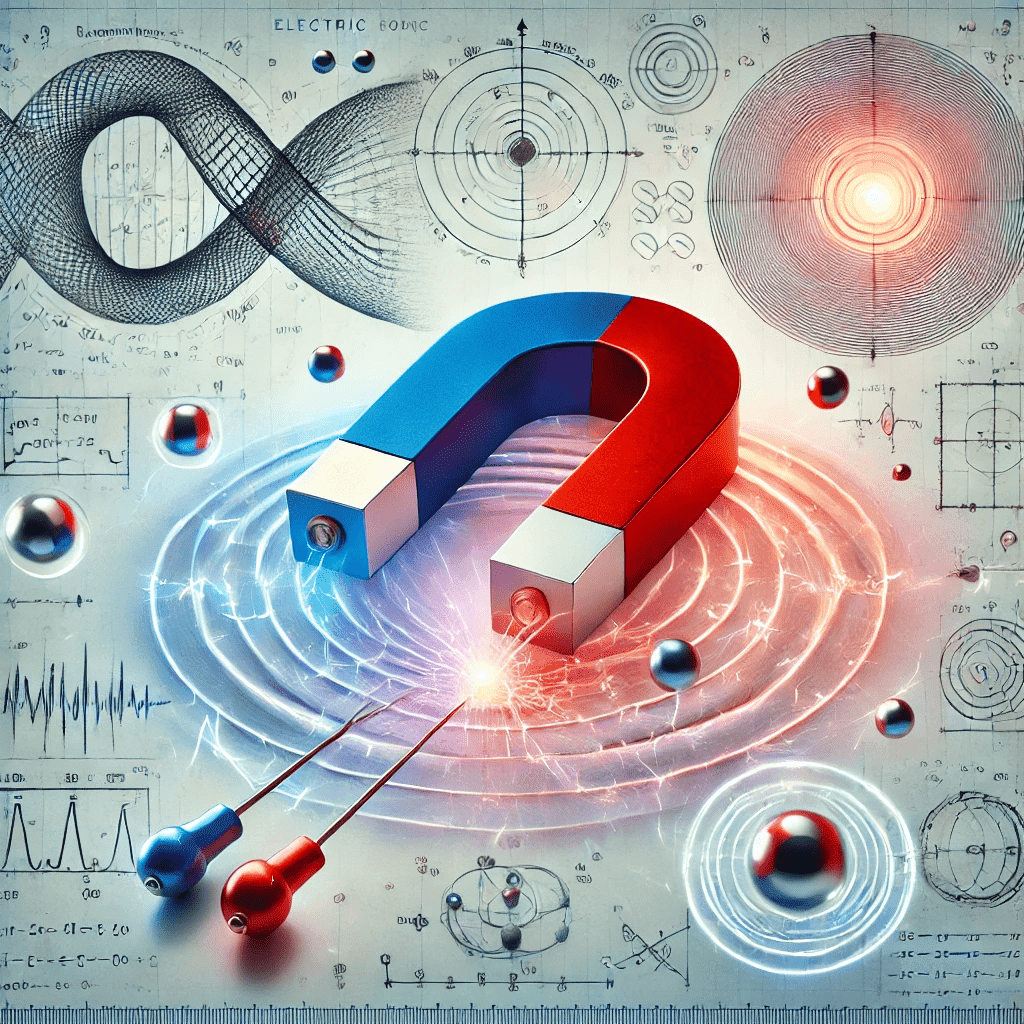
\includegraphics[width=2cm]{EMInteractions}};
\end{frame}

% ============================== Слайд ## ===================================
\begin{frame}{Зміст лекції}{}
	\tableofcontents
\end{frame}
% ===========================================================================


\section{Сили (взаємодії) в природі}


% ============================== Слайд ## ===================================
\begin{frame}{Сили (взаємодії) в природі}{}\footnotesize
	\begin{center}
		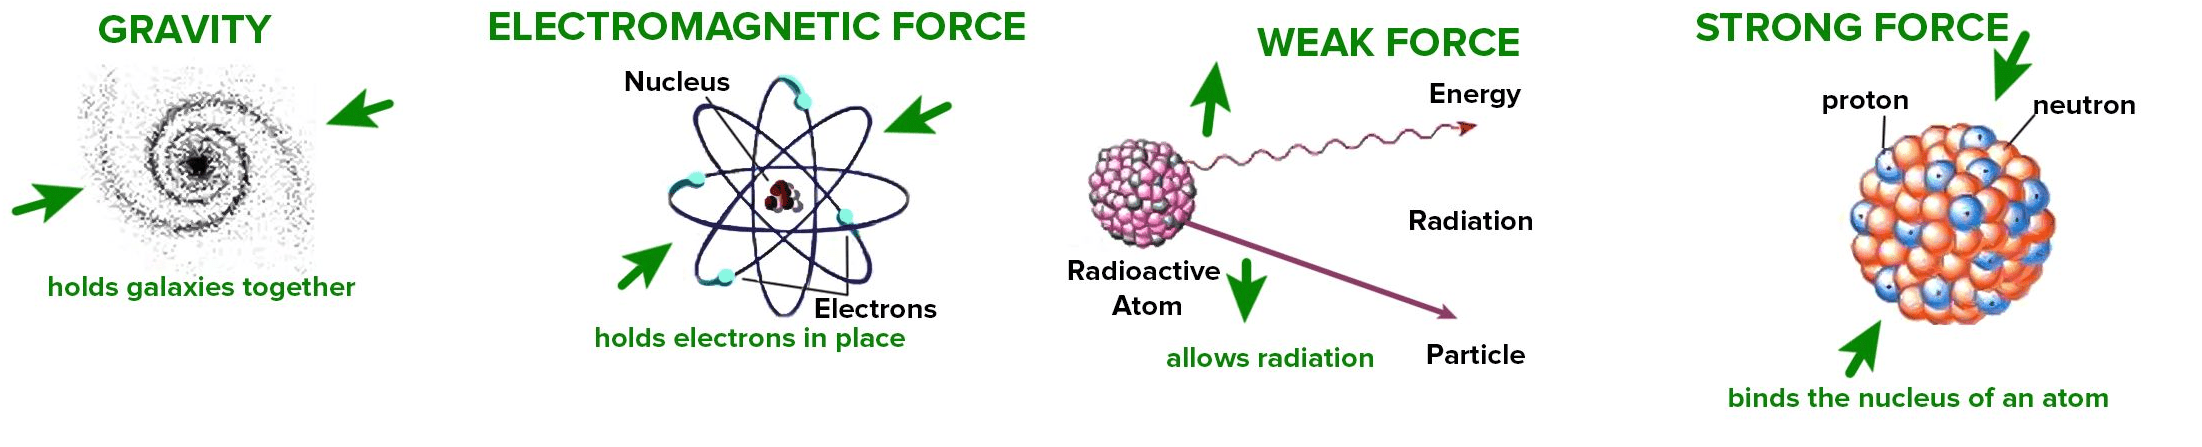
\includegraphics[width=\linewidth]{forces}
	\end{center}
	\begin{center}
		\begin{tblr}{
			colspec = {Q[l, m]Q[c, m, 1.5cm]Q[c, m, 2cm]Q[c, m]Q[c, m]},
			hlines,
			vlines,
			row{1} = {c, bg=cyan, fg=white, font=\bfseries},
			row{3} = {bg=yellow!60},
			}
			Взаємодія       & Джерело           &
			Ефект           & Радіус дії        &
			Інтенсивність                                                                               \\
			Гравітація      & Маса              & \alert{Всі} тіла притягуються          & $\infty$   &
			$10^{-38}$
			\\
			Електромагнітна & Електричний заряд & Заряджені тіла притягуються і
			відштовхуються  & $\infty$          & $10^{-2}$                                             \\
			Слабка ядерна   & Слабкий заряд     & Розпад більш масивних частинок до менш
			масивних        & $10^{-16}$ см     & $10^{-10}$                                            \\
			Сильна ядерна   & Кольоровий заряд  & Притягування кварків                   & $10^{-13}$
			см              & 1
		\end{tblr}
	\end{center}
\end{frame}
% ===========================================================================



\section{Основні поняття}


% ============================== Слайд ## ===================================
\begin{frame}{Електромагнітна взаємодія}{}
	\begin{onlyenv}<1>
		\begin{block}{}\justifying
			\alert{Електромагнітна взаємодія} є одним із фундаментальних типів
			взаємодій. Вона здійснюється на відстані, без прямого контакту
			взаємодіючих тіл, і передається за допомогою особливого носія ---
			\alert{електромагнітного поля}.
		\end{block}
		\begin{block}{}
			\alert{Електромагнітним полем} називається область простору, де діють
			електричні та магнітні сили.
		\end{block}
		\begin{block}{}
			Поле \alert{створюється} електричними \textit{зарядами} і \alert{діє}
			на \textit{заряди}.
		\end{block}
		\begin{block}{}\justifying
			\alert{Електричний заряд} --- це міра взаємодії \alert{зарядженого
				тіла з полем}. Фактично, заряд визначає інтенсивність взаємодії
			заряджених тіл.
		\end{block}
	\end{onlyenv}
	\begin{onlyenv}<2>
		\begin{block}{}
			\begin{tikzpicture}[pencildraw/.style={ %
							decorate,
							decoration={random steps,segment length=2pt,amplitude=1pt}
						} %
				]
				\node[align=justify, drop shadow,
					preaction={fill=black,opacity=.5},
					pencildraw,draw,fill=white,text width=1\linewidth,inner sep=2mm]
				{Якби у вашому тілі або в тілі вашого сусіда (який стоїть від вас на
					відстані витягнутої руки) електронів виявилося б всього на 1\% більше, ніж
					протонів, то сила вашого відштовхування була б неймовірно великою.\\[1ex]
					Наскільки великою? Достатньою, щоб підняти хмарочос? Більше! Достатньою,
					щоб підняти гору Еверест? Більше!\\[1ex]
					Сили відштовхування вистачило б, щоб
					підняти «вагу», що дорівнює вазі нашої Землі!\\[1em]
					\hfill{ Р. Фейнман в книзі <<Фейнманівські лекції з фізики>>}.
				};
			\end{tikzpicture}
		\end{block}
		\tikz[remember picture,overlay] \node[opacity=0.5,inner sep=0pt,
			anchor=south west] at (current page.south
		west){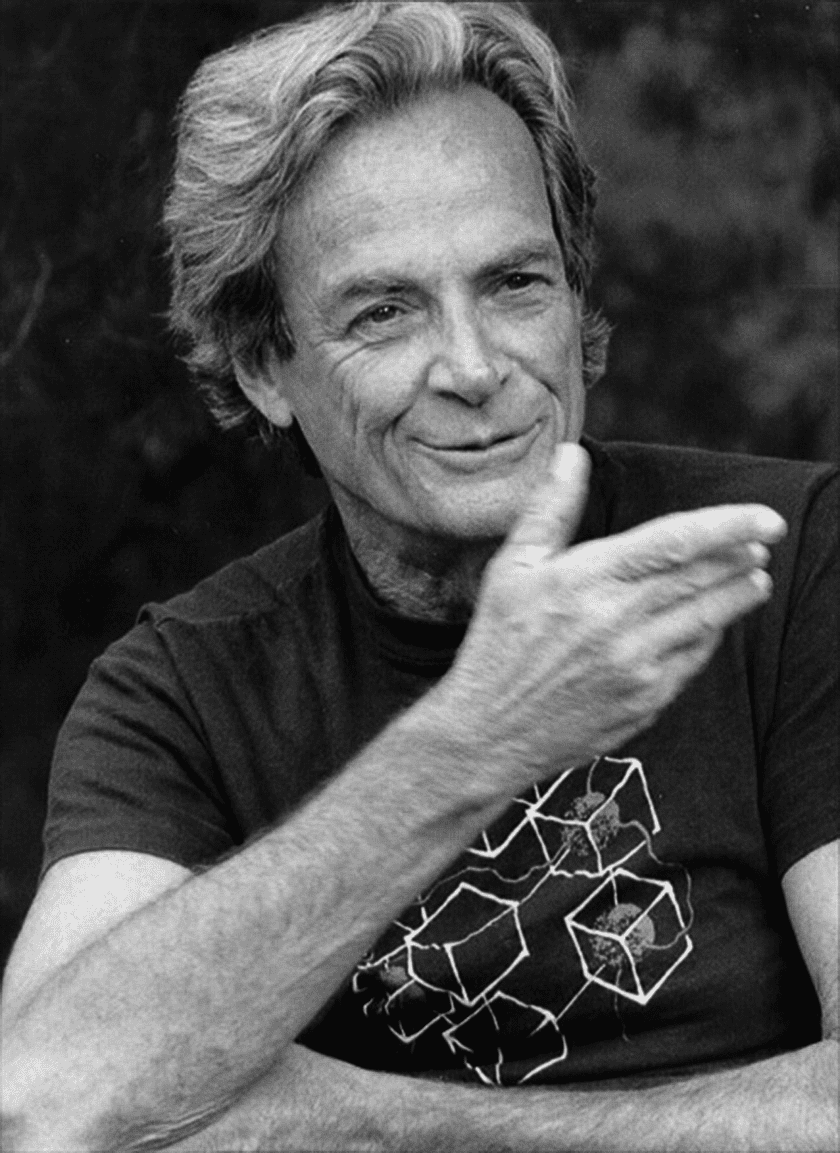
\includegraphics[width=2cm]{Fey}};
	\end{onlyenv}
\end{frame}
% ===========================================================================




% ============================== Слайд ## ===================================
\begin{frame}{Системи одиниць}{}
	\tikz[remember picture,overlay] \node[opacity=0.7,inner sep=0pt,
		anchor=north west] at (current page.north
	west){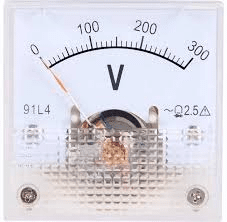
\includegraphics[width=2cm]{units}};
	\begin{block}{}\centering
		За основну в курсі прийнято \alert{гауссову систему одиниць}.
	\end{block}
	\begin{center}
		\begin{tblr}{
			colspec = {Q[l, m]X[c, m]X[c, m]},
			hlines,
			vlines,
			row{1} = {c, bg=cyan, fg=white, font=\bfseries},
			}
			{Характеристика} & {Система СІ}                           & {Гауссова система}      \\
			Основні одиниці  & метр, кілограм, секунда  (МКС),  ампер &
			сантиметр, грам, секунда
			(СГС)                                                                               \\
			Сила струму      & Ампер                                  & Відсутня окрема одиниця \\
			Застосування     & Широке використання в техніці та науці & Теорія
			поля, теоретична фізика                                                             \\
		\end{tblr}
	\end{center}

	\begin{alertblock}{}\justifying
		Гауссова система СГС до теперішнього часу залишається найкращою у фізиці.
		Для фізика значно легше виконати всі обчислення в гаусовій системі і лише
		наприкінці, якщо це потрібно, зробити перерахунок до практичних одиниць.
	\end{alertblock}
\end{frame}
% ===========================================================================


% ============================== Слайд ## ===================================
\begin{frame}{Деякі фізичні константи в гауссовій системі}\small
	\begin{tblr}{
		colspec={X[l,m]Q[c,m]Q[l,m]},
		row{1} = {1.5em, c, azure2, fg=white,font=\bfseries\sffamily},
		row{odd[2-Z]}={gray9},
		row{2-Z}={1.7em},
		cell{1}{4}={mode=text},
		hlines={azure3},
		vlines={azure3},
		vline{2-4}={1}{white},
		hline{2}={white}
		}
		Константа                  & Символ  &
		Значення                                                              \\
		Швидкість світла у вакуумі & $c$     & $2.997 924 58 \cdot 10^{10}$
		см/с                                                                  \\
		Гравітаційна стала         & $G$     & $6.674 28 \cdot 10^{-8}$
		см$^3$/(г$\cdot$c$^2$)                                                \\
		Стала Планка               & $\hbar$ & $1.054 5716 \cdot 10^{-27}$
		ерг$\cdot$с                                                           \\
		Елементарний заряд         & $e$     & $4.803 204 27  \cdot 10^{-10}$
		Фр                                                                    \\
		Маса електрона             & $m_e$   & $9.109 382 15 \cdot 10^{-28}$
		г                                                                     \\
		Маса протона               & $m_p$   & $1.672 621 9 \cdot 10^{-30}$
		г                                                                     \\
		Борівський радіус          & $a_0$   & $5.291 772 0859 \cdot 10^{-9}$
		см                                                                    \\
		Магнетон Бора              & $\mu_B$ & $9.274 009 15 \cdot 10^{-21}$
		ерг/Гс                                                                \\
		Електрон-Вольт             & еВ      & $1.602\cdot 10^{-12}$
		ерг
	\end{tblr}
\end{frame}
% ===========================================================================

% ============================== Слайд ## ===================================
\begin{frame}{Електричний заряд}
	\framesubtitle<1>{Досліди Міллікена}
	\framesubtitle<2>{Властивості}
	\begin{alertblock}{}\centering
		Заряд --- фундаментальна властивість деяких видів елементарних
		частинок.
	\end{alertblock}
	\begin{onlyenv}<1>
		\begin{columns}
			\begin{column}{0.4\linewidth}
				\begin{figure}
					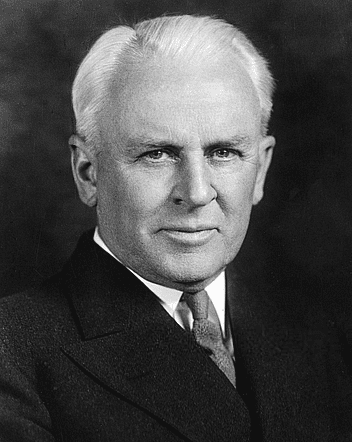
\includegraphics[width=0.62\linewidth]{Millikan-1920s}
					\caption{Роберт Міллікен}
				\end{figure}
			\end{column}
			\begin{column}{0.4\linewidth}
				\begin{figure}
					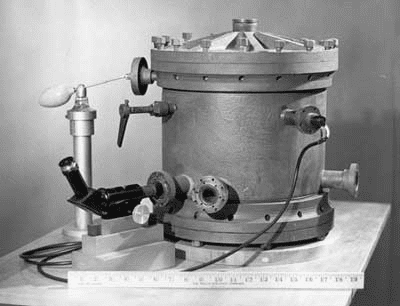
\includegraphics[width=1\linewidth]{Millikan-chamber}
					\caption{Установка Міллікена}
				\end{figure}
			\end{column}
		\end{columns}
		\begin{block}{}\justifying
			Експеримент із вимірювання елементарного електричного заряду,
			здійснений 1909 року Робертом Ендрюсом Міллікеном та Гарві
			Флетчером. В результаті було встановлено дискретність електричного
			заряду та визначив величину заряду електрона з точністю до 1\%.
			\href{https://www.youtube.com/watch?v=5LC4-ct_1-M}{Відео: Досліди Міллікена та Йоффе}
		\end{block}
	\end{onlyenv}

	\begin{onlyenv}<2>
		\begin{enumerate}\justifying
			\item Дискретність заряду.

			      \begin{flushleft}\small
				      Дослідним шляхом було встановлено, що в природі існують \alert{заряди двох типів}, які умовно ділять на \alert{позитивні} та
				      \alert{негативні}. Позитивний заряд несуть, наприклад, протони, а негативний --- електрони. У природі заряд змінюється (переноситься)
				      дискретно, причому будь-який ненульовий заряд кратний деякому елементарному заряду, що чисельно дорівнює заряду електрона:
				      \begin{equation*}
					      e = 4.803 \cdot 10^{-10}\ \text{Фр} = 1.602 \cdot 10^{-19}\ \text{Кл}.
				      \end{equation*}
			      \end{flushleft}

			\item Збереження заряду.

			      \begin{flushleft}\small
				      Заряд --- це величина, що \alert{зберігається}. Позитивні й негативні заряди можуть народжуватися в рівних кількостях або взаємно
				      знищувати один одного. При цьому сумарний електричний заряд речовини не змінюється.
			      \end{flushleft}
			\item Релятивістська інваріантність заряду.

			      \begin{flushleft}\small
				      Величина електричного заряду однакова відносно різних систем відліку. Іншими словами, величина заряду не залежить від швидкості.
			      \end{flushleft}
		\end{enumerate}
	\end{onlyenv}
\end{frame}
% ===========================================================================

% ============================== Слайд ## ===================================
\begin{frame}{Як заряджають тіла?}{Трибоелектричний ефект}
	\tikz[remember picture,overlay] \node[opacity=0.7,inner sep=0pt,
		anchor=south east] at (current page.south
	east){
\includegraphics[width=3cm]{Tribocat}};

	\tikz[remember picture,overlay] \node[opacity=0.7,inner sep=0pt,
		anchor=north west] at ([yshift=-1.5cm]current page.north
	west){
\includegraphics[width=5cm]{charging-by-friction}};

	\tikz[remember picture,overlay] \node[opacity=0.7,inner sep=0pt,
		anchor=north east] at ([yshift=-1.7cm]current page.north
	east){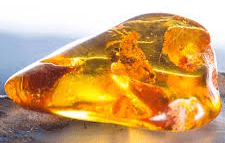
\includegraphics[width=3cm]{Amber}};

	\begin{onlyenv}<1>
		\begin{block}{}
			\alert{Трибоелектричний ефект} --- поява електричних зарядів у
			матеріалі через тертя.
		\end{block}

		\begin{block}{}\justifying
			Деякі матеріали стають електрично зарядженими після того, як вони
			входять у
			фрикційний контакт з іншим матеріалом.
		\end{block}

		\begin{exampleblock}\justifying\small
			Слово <<\alert{електрика}>> походить від грецького
			<<$\eta\lambda\varepsilon\kappa\tau\rho o \nu$>>
			(\alert{електрон}), що означає <<\alert{бурштин}>>. Люди помітили,
			що бурштин, натертий об хутро, притягує дрібні предмети, і це
			явище згодом стало основою для дослідження електричних явищ.
		\end{exampleblock}
	\end{onlyenv}

	\begin{onlyenv}<2>
		\begin{block}{}\justifying
			Матеріали, що виявляють трибоелектричний ефект, прийнято
			розташовувати в \alert{трибоелектричний ряд}, один кінець якого є
			позитивним, а інший --- негативним. Під час тертя пари матеріалів
			з ряду, матеріал, розташований ближче до позитивного кінця ряду,
			зарядиться позитивно, а інший --- негативно.

			\bigskip

			ряд Фарадея: ($+$) хутро, фланель, слонова кістка, пір'я, гірський
			кришталь, флінтглас, паперова тканина, шовк, дерево, метали, сірка
			($-$).
		\end{block}
	\end{onlyenv}
\end{frame}
% ===========================================================================


% ============================== Слайд ## ===================================
%\begin{frame}{Електроскоп та електрофорна
%		машина}{Відеодемонстрації}\begin{columns}
%		\begin{column}{0.5\linewidth}
%			\begin{figure}
%
%\href{https://www.youtube.com/watch?v=3VpRqhljk5w}{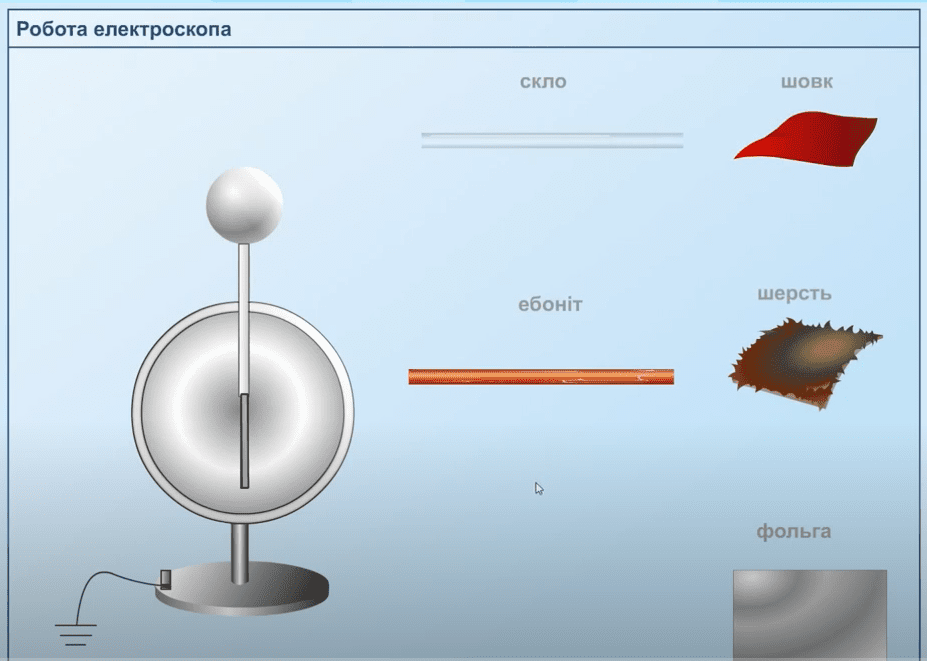
\includegraphics[width=4cm]{VideoElectroscope}}
%				\caption{Як працює електроскоп}
%			\end{figure}
%		\end{column}
%		\begin{column}{0.5\linewidth}
%			\begin{figure}
%
%\href{https://youtu.be/MzqQ4Fc0RTg}{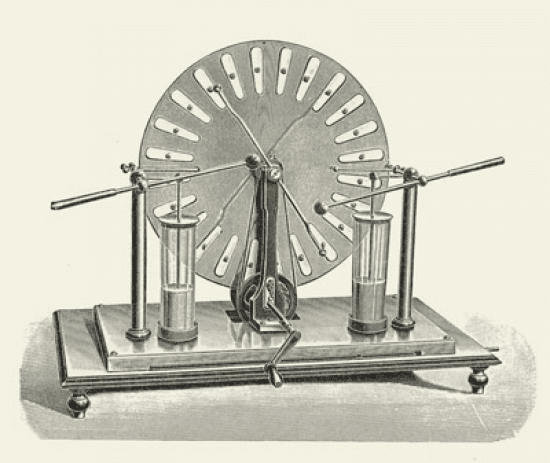
\includegraphics[width=4cm]{WimshurstElectricMachine}}
%				\caption{Електрофорна машина}
%			\end{figure}
%		\end{column}
%	\end{columns}
%
%\end{frame}
% ===========================================================================

% ============================== Слайд ## ===================================
\begin{frame}{Крутильні терези}{Досліди Кавендіша та Кулона}
	\begin{columns}
		\begin{column}{0.4\linewidth}
			\begin{center}
				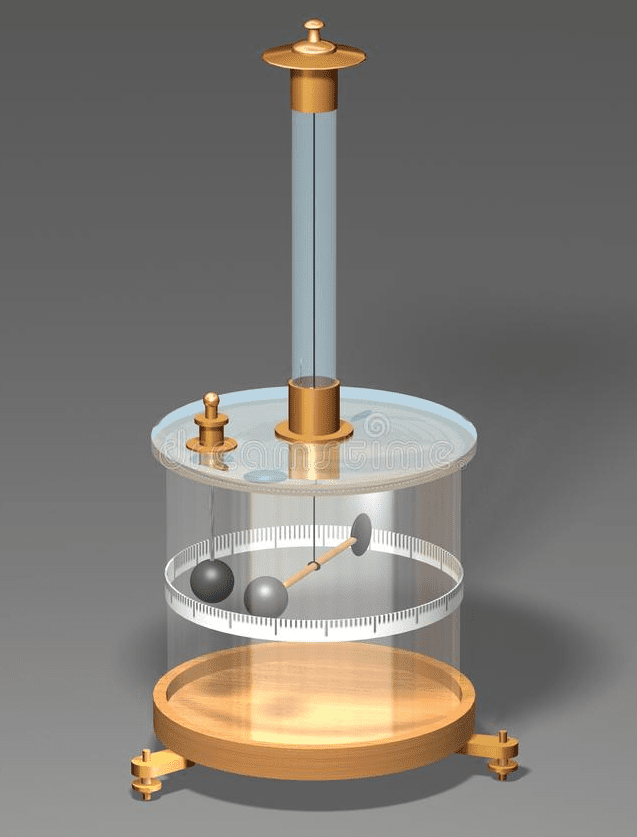
\includegraphics[width=\linewidth]{ColumbTorsiomBalance}
			\end{center}
		\end{column}
		\begin{column}{0.6\linewidth}\justifying
			\alert{Крутильні (торсіонні) терези} --- це прилад для вимірювання
			дуже слабких сил,
			винайдений Шарлем Кулоном в 1777 році.

			\medskip

			Найвідоміші випадки  використання:
			\begin{enumerate}\justifying
				\item вимірювання Кулоном електростатичної сили між зарядами
				      для встановлення закону Кулона;
				\item в експерименті Генрі Кавендішем у 1798 році для
				      вимірювання сили тяжіння між двома масами для обчислення маси
				      Землі, що згодом дозволило отримати значення гравітаційної
				      сталої.
			\end{enumerate}
		\end{column}
	\end{columns}
	\vfill

	\href{https://www.youtube.com/watch?v=5pmkBq3eDcw}{\small Відео:
		Досліди Кавендіша з крутильними терезами}
\end{frame}
% ===========================================================================



% ============================== Слайд ## ===================================
\begin{frame}{Закон Кулона}{}
	\tikz[remember picture,overlay] \node[opacity=0.5,inner sep=0pt,
		anchor=south east] at (current page.south
	east){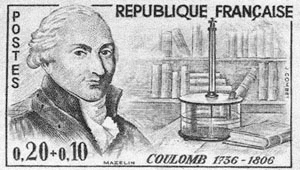
\includegraphics[width=3cm]{coulombpostmark}};
	\begin{block}{}\justifying
		Експериментально встановлено, що заряди одного знака (однойменні
		заряди) \alert{відштовхуються}, а заряди різного знака (різнойменні
		заряди) --- \alert{притягуються}.
	\end{block}

	\begin{block}{}\justifying
		\alert{Точковим} називається такий заряд, розмірами та формою якого в
		умовах, що розглядаються, можна знехтувати.
	\end{block}

	\begin{block}{}\justifying
		Закон, установлений Ш. Кулоном у 1785 р., стверджує, \alert{що сила,
			що діє на точковий заряд} $q_1$ з боку точкового заряду $q_2$:
		\begin{equation*}
			\tcbhighmath{
				\vec{F}_{12} = \frac{q_1 q_2}{r^2}\frac{\vec{r}_{12}}{r}.
			}
		\end{equation*}
	\end{block}

	\begin{center}
		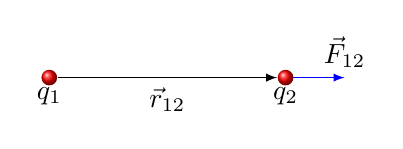
\begin{tikzpicture}[>=latex, scale=1.5]
	\node [circle, ball color=red, inner sep=2pt] (q1) at (-1,0) {};
	\node [circle, ball color=red, inner sep=2pt] (q2) at (1,0) {};

	\node[below] at (q1) {$q_1$};
	\node[below] at (q2) {$q_2$};
	\draw[->] (q1) -- node[below] {$\vec{r}_{12}$} (q2);

	\draw[->, blue] (q2) -- ++(0.5,0) node[above, text=black]
	{$\vec{F}_{12}$};
\end{tikzpicture}
	\end{center}

\end{frame}
% ===========================================================================



% ============================== Слайд ## ===================================
\begin{frame}{Експериментальні перевірки закону Кулона}{}\small
\begin{block}{}\justifying
Якщо припустити, що закон взаємодії точкових зарядів відрізняється від закону оберненого квадрату, наприклад:
\begin{equation*}
F = \frac{q_1 q_2}{r^{2 + \epsilon}},
\end{equation*}
де $|\epsilon| \ll 1$, то при збереженні принципу суперпозиції це призводить до якісних змін у поведінці зарядів у
провідниках. У випадку кулонівської взаємодії у стаціонарних умовах заряди зосереджуються на поверхні провідника, а всередині зарядів немає.
Однак, якщо виконується формула з $\epsilon$, то можна показати, що у провіднику виникає ненульова густина заряду у стаціонарних умовах.
\end{block}
\begin{columns}
	\begin{column}{0.4\linewidth}
         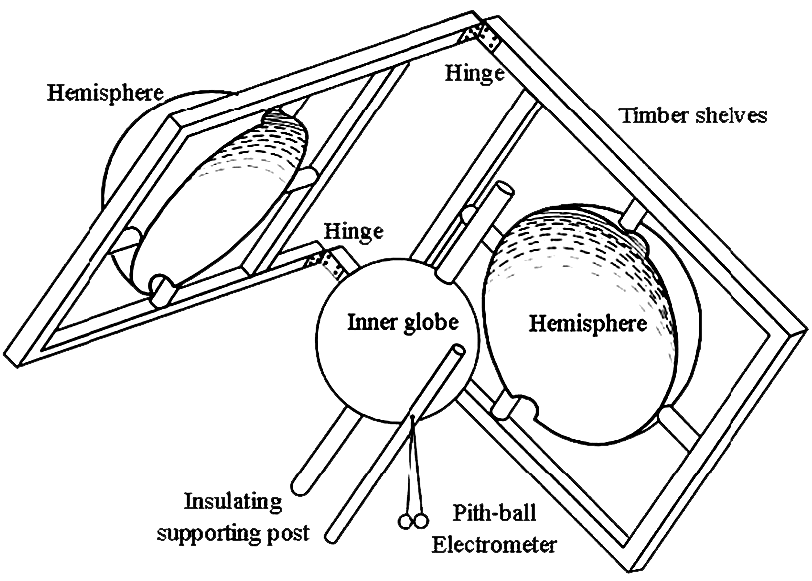
\includegraphics[width=\linewidth]{cavindesh_exp}
	\end{column}
	\begin{column}{0.6\linewidth}
 \begin{block}{}\justifying\footnotesize
    Цю обставину було використано для отримання обмеження на $\epsilon$. На попередньо заряджену провідну кулю накладали дві провідні напівсфери, які
щільно прилягали одна до одної, утворюючи майже суцільну поверхню. У цій системі, у разі кулонівської взаємодії ($\epsilon = 0$), весь заряд
переходить на зовнішні напівсфери. Якщо ж $\epsilon \neq 0$, всередині кулі залишається заряд (тим менший, чим менше $\epsilon$), який можна
виміряти за допомогою чутливого електрометра після зняття напівсфер. Цей експеримент неодноразово повторювався із поступовим підвищенням точності. У
1983 році було отримано обмеження:
\begin{equation*}
|\epsilon| < 10^{-16} \text{–} 10^{-17}.
\end{equation*}
\end{block}
	\end{column}
\end{columns}

\end{frame}
% ===========================================================================



% ============================== Слайд ## ===================================
\begin{frame}{Напруженість електричного поля}{}
	\begin{block}{}\justifying
		Для дослідження поля, створюваного будь-якими зарядами
		(зарядженими тілами), можна використовувати \alert{пробні заряди}.

		\bigskip

		\alert{Пробним} називається такий невеликий за величиною точковий
		заряд, який не виробляє помітного перерозподілу зарядів,
		що створюють досліджуване поле.
	\end{block}

	\begin{block}{}\justifying
		Дослідним шляхом установлено, що якщо помістити в електричне
		поле пробний заряд $q$ то відношення сили F, що діє на цей
		заряд, до величини заряду не залежить від величини заряду. Отже,
		відношення $F/q$ характеризує поле, але не заряд.
	\end{block}

	\begin{block}{}
		\alert{Напруженістю електричного поля} в \emph{деякій точці}
		називається сила, що діє на одиничний точковий заряд:
		\begin{equation*}
			\vec{E} = \frac{\vec{F}}{q}, \quad \vec{F} = q\vec{E}.
		\end{equation*}
	\end{block}
\end{frame}
% ===========================================================================


% ============================== Слайд ## ===================================
\begin{frame}{Напруженість поля точкового заряду}{}
	Відповідно до закону Кулона напруженість поля точкового
	заряду $Q$ дорівнює:
	\begin{equation*}
		\tcbhighmath{
			\vec{E} = \frac{Q}{r^2}\ \frac{\vec{r}}{r}.
		}
	\end{equation*}
		\begin{columns}
		\begin{column}{0.5\linewidth}\centering
			\begin{tikzpicture}[>=latex, transform shape, scale=1.5]
				\node [circle, ball color=red, inner sep=0pt, text=white,
					font=\scriptsize] (qp) at (0,0) {$+$};
				\node[circle, inner sep=0.75pt, fill] (P) at (1, 2) {};
				\node[left] at (P) {$P$};

				\node[below=5pt] at (qp) {$Q$};

				\draw[->] (qp) -- node[left] {$\vec{r}$} (P);

				\draw[->, red, thick] let \p1=(qp), \p2=(P) in (P) --
				++({atan(
						(\y2-\y1)
						/ (\x2 - \x1) )}:0.5) node[right] {$\vec{E}$};
			\end{tikzpicture}
		\end{column}
		\begin{column}{0.5\linewidth}\centering
			\begin{tikzpicture}[>=latex, transform shape, scale=1.5]
				\node [circle, ball color=blue, inner sep=1.2pt, text=white]
				(qn) at
				(0,0) {\tikz\draw[thick] (0,0) -- ++(0.1,0);};
				\node[circle, inner sep=0.75pt, fill] (P) at (1, 2) {};

				\node[below=5pt] at (qn) {$Q$};

				\node[left] at (P) {$P$};

				\draw[->] (qn) -- node[left] {$\vec{r}$} (P);

				\path let \p1=(qn), \p2=(P) in (P) --
				++({atan(  (\y2-\y1) / (\x2 - \x1) )}:0.5);

				\draw[->, blue, thick] let \p1=(qn), \p2=(P) in (P) --
				++({180+atan( (\y2-\y1)
						/ (\x2 - \x1) )}:0.5) node[below right] {$\vec{E}$};
			\end{tikzpicture}
		\end{column}
	\end{columns}

\end{frame}
% ===========================================================================

% ============================== Слайд ## ===================================
\begin{frame}{Принцип суперпозиції}{}

	\begin{onlyenv}<1>
		\begin{block}{}\justifying
			Сила, що діє на заряд $q$ з боку системи інших зарядів, дорівнює
			векторній сумі сил, що незалежно діють на розглянутий заряд з боку
			кожного із зарядів системи:
			\begin{equation*}
				\vec{F} = \sum_{i=1}^{n} \vec{F}_i
			\end{equation*}
		\end{block}
	\end{onlyenv}

	\begin{onlyenv}<1-2>
		\begin{block}{}\justifying
			Оскільки $\vec{F}_i = q\vec{E}_i$, то напруженість поля в цій точці
			також
			дорівнює векторній сумі напруженостей полів, незалежно створюваних
			у цій точці кожним із зарядів системи:
			\begin{equation*}
				\vec{E} = \sum_{i=1}^{n} \vec{E}_i
			\end{equation*}
		\end{block}
	\end{onlyenv}

	\begin{onlyenv}<2>
		\begin{center}
						\begin{tikzpicture}[>=latex, transform shape, scale=1.5]

				\def\qp{1.2}
				\def\qn{0.5}
				\node [circle, ball color=red, inner sep=0pt, text=white,
					font=\scriptsize] (q1) at
				(-1,0.5)
				{$+$};
				\node [circle, ball color=blue, inner sep=1pt, text=white]
				(q2) at
				(2,0) {\tikz\draw[thick] (0,0) -- ++(0.1,0);};

				\node[inner sep = 0.5pt, fill, circle] (P) at (0.2, 1) {};
				\node[above] at (P) {$P$};


				\draw (q1) -- (P) (q2) -- (P);

				\draw[->, red] let \p1=(q1), \p2=(P) in (P) --
				++({ atan((\y2 - \y1)/(\x2 - \x1) ) }:\qp) coordinate (E1)
				node[above]
					{$\vec{E}_1$};

				\draw[->, blue] let \p1=(q2), \p2=(P) in (P) --
				++({ atan((\y2 - \y1)/(\x2 - \x1) ) }:\qn) coordinate (E2)
				node[below left]
					{$\vec{E}_2$};

				\draw[dashed]  let \p1=(q2), \p2=(P) in (E1) -- ++({ atan((\y2
						- \y1)/(\x2 - \x1) ) }:\qn) coordinate (E);

				\draw[dashed]  let \p1=(q1), \p2=(P) in (E2) -- ++({ atan((\y2
						- \y1)/(\x2 - \x1) ) }:\qp);

				\draw[->] (P) -- (E) node[right] {$\vec{E}$};

			\end{tikzpicture}
		\end{center}
	\end{onlyenv}
\end{frame}
% ===========================================================================


% ============================== Слайд ## ===================================
\begin{frame}{Силові лінії}{}
	\begin{block}{}
		\alert{Силовою лінією} називається така лінія, у кожній точці якої
		напрямок дотичної до неї збігається з напрямком напруженості поля в тій
		самій точці.
	\end{block}
	\begin{columns}
		\begin{column}{0.45\linewidth}
			\begin{center}
								\begin{tikzpicture}[x=1.5cm,y=1.4cm]
					\tikzset{
						draw tangents/.style={decorate,decoration={
										markings,mark=between positions 0 and
										1 step
										.2 with
											{\draw[-latex,black,thin] (0,0) --
												(1cm,0)
												node[above] {$\vec{E}$};},
									}
							}
					}
					\draw[red,thick,postaction=draw tangents]
					(0,0) to[out=45, in=135] (3,0);
				\end{tikzpicture}
			\end{center}
		\end{column}
		\begin{column}{0.45\linewidth}
			\begin{block}{}
				Стрілки вказують напрямок електричного поля в різних
				точках цієї лінії.
			\end{block}
		\end{column}
	\end{columns}
	\begin{center}
		\includegraphics[width=1\linewidth]{fieldlines}
	\end{center}
\end{frame}
% ===========================================================================


% ============================== Слайд ## ===================================
\begin{frame}{Електричний момент системи зарядів}{}
	\begin{block}{}\justifying
		Для довільної системи зарядів дипольний момент визначається формулою:
		\begin{equation*}
			\vec{p} = \sum_{i=1}^{n}q_i\vec{r}_i,
		\end{equation*}
		де $\vec{r}_i$ --- радіус-вектор $i$-го заряду.

	\end{block}

	\begin{exampleblock}{}\justifying\small
		У загальному випадку ця
		величина залежить від вибору початку відліку. Однак якщо система
		загалом електронейтральна $\sum_{i=1}^{n} q_i = 0$, то
		дипольний момент $\vec{p}$ визначений однозначно.
	\end{exampleblock}

	\begin{columns}
		\begin{column}{0.7\linewidth}
			\begin{overprint}
				\onslide<1>
				\begin{block}{}\justifying\small
					\alert{Елементарний диполь} --- система, що складається з
					двох точкових зарядів $q$, однакових за величиною і
					протилежних за знаком.

					\medskip

					\alert{Плече диполя} --- вектор ($\vect{\ell}$), що йде від <<$-$>> заряду до
					<<$+$>>, довжина якого дорівнює відстані між зарядами.

					\medskip

					\alert{Дипольним моментом} диполя називається вектор
					\begin{equation*}
						\vec{p} = q\vec{\ell}
					\end{equation*}.
				\end{block}
				\onslide<2>
				\begin{alertblock}{}\centering
					Диполь --- модель реальних об'єктів!
				\end{alertblock}

				\begin{block}{}\justifying\small
					\alert{Жорсткий диполь} --- диполь із фіксованою відстанню між зарядами, що не
					змінюється під зовнішніми впливами.

					\medskip

					\alert{Пружний диполь} --- диполь, де відстань між зарядами змінюється під зовнішніми
					впливами, і дипольний момент може змінюватися.
				\end{block}
			\end{overprint}
		\end{column}
		\begin{column}{0.3\linewidth}\centering
			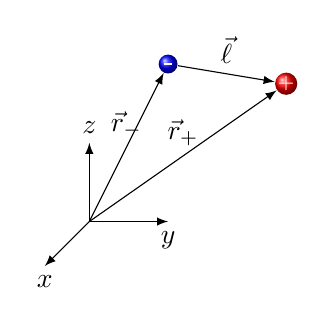
\begin{tikzpicture}[>=latex]
	\draw[->] (0,0) -- ++(1, 0) node[below] {$y$};
	\draw[->] (0,0) -- ++(0, 1) node[above] {$z$};
	\draw[->] (0,0) -- (-135:0.8) node[below] {$x$};

	\node [circle, ball color=blue, inner sep=1.2pt, text=white]
	(qn) at (1,2) {\tikz\draw[thick] (0,0) -- ++(0.1,0);};

	\node [circle, ball color=red, inner sep=0pt, text=white,
		font=\scriptsize] (qp) at (2.5,1.75) {$+$};

	\draw[->] (0,0) -- (qp) node[pos=0.5, above] {$\vec{r}_+$};
	\draw[->] (0,0) -- (qn) node[pos=0.5, above] {$\vec{r}_-$};
	\draw[->] (qn) -- node[above] {$\vec{\ell}$} (qp);
\end{tikzpicture}
		\end{column}
	\end{columns}
\end{frame}
% ===========================================================================




% ============================== Слайд ## ===================================
\begin{frame}{Дипольні моменти деяких полярних молекул}

	\begin{block}{}\justifying
		Дипольний момент виникає внаслідок різної електронегативності атомів, що складають
		молекулу, та
		розташуванню їх в просторі.
	\end{block}
	\begin{exampleblock}{}\justifying\small
		Дебай (позначається як \textit{Д} або \textit{D}) --- позасистемна одиниця вимірювання
		електричного дипольного моменту молекул. Одиниця виміру названа на честь фізика П. Дебая.
		\begin{equation*}
			1\ \text{Дебай} = 10^{-18}\ \text{Фр}\cdot\text{см}.
		\end{equation*}
		Більшість полярних молекул має дипольний момент порядку $1$ Д. Одиниця застосовується у
		фізичній хімії, атомній і молекулярній фізиці.
	\end{exampleblock}

	\begin{overprint}\centering
		\onslide<1>
		\begin{columns}
	\begin{column}{0.5\linewidth}\centering
		\begin{tikzpicture}[>=latex]
			\node[circle, draw=blue, ball color=blue!50, inner sep=0.28cm, text=blue] (O) at
			(0,0)
			{\tikz\draw[blue, thick] (0,0) -- ++(0.4, 0);};
			\node[below=15pt] at (O) {\ce{O^{2-}}};
			\node[circle, draw=red, ball color=red!50, inner sep=0.16cm, text=blue] (H1) at
			({90+105/2}:1)
			{$+$};
			\node[left=15pt] at (H1) {\ce{H^{+1}}};
			\node[circle, draw=red, ball color=red!50, inner sep=0.16cm, text=blue] (H2) at
			({90-105/2}:1)
			{$+$};
			\node[right=15pt] at (H2) {\ce{H^{+1}}};
			\draw[dashed, gray] (0, 0) -- ({90+105/2}:2);
			\draw[dashed, gray] (0, 0) -- ({90-105/2}:2);

			\draw[<->] (0, 0) ++({90-105/2}:1.8) arc({90-105/2}:{90+105/2}:1.8) node[pos=0.5,
					fill=white,
					font=\scriptsize]
				{$105^\circ$};

			\draw[->, red, ultra thick] (0,0) -- ++(0, 1.5) node[right] {$\vect{p}$};
		\end{tikzpicture}
        \begin{block}{}\footnotesize\centering
            Дипольний момент молекули \ce{H2O} $p = 1.84$ D
        \end{block}
	\end{column}
	\begin{column}{0.5\linewidth}\centering
    \begin{tikzpicture}[>=latex]
            \node[circle, draw=blue, ball color=blue!50, inner sep=0.28cm, text=blue] (N) at
			(0,0) {\tikz\draw[blue, thick] (0,0) -- ++(0.4, 0);};
        \node[above=15pt] at (N) {\ce{O}};
        \node[circle, draw=red, ball color=red!50, inner sep=0.16cm, text=blue] (H1) at
   				(225:1.2) {$+$};
        \node[circle, draw=red, ball color=red!50, inner sep=0.16cm, text=blue] (H2) at
			(280:1.8) {$+$};
        \node[circle, draw=red, ball color=red!50, inner sep=0.16cm, text=blue] (H3) at
   				(-45:1.2) {$+$};
        \draw[thick] (O) -- (H1) (O) -- (H2) (O) -- (H3);
        \draw[dashed] (H1) -- (H2) -- (H3) -- (H1);
       	\draw[->, red, ultra thick] (0,0) -- ++(0, -1.2) node[left] {$\vect{p}$};
    \end{tikzpicture}
        \begin{block}{}\footnotesize\centering
            Дипольний момент молекули \ce{NH3} $p = 1.46$ D
        \end{block}
	\end{column}
\end{columns}
		\onslide<2>
		\begin{tblr}{
			colspec={X[c, m]X[c,m]},
			row{1} = {c, m, fg=white, bg=cyan},
			hlines,
			vlines
			}
			Молекула                   & Дипольний момент (Дебай) \\
			Вода (\ce{H2O})            & 1.84                     \\
			Аміак (\ce{NH3})           & 1.46                     \\
			Вуглекислий газ (\ce{CO2}) & 0.00                     \\
			Хлороводень (\ce{HCl})     & 1.08                     \\
			Метанол (\ce{CH3OH})       & 1.70                     \\
		\end{tblr}
	\end{overprint}
\end{frame}
% ===========================================================================



% ============================== Слайд ## ===================================
\begin{frame}{Виникнення дипольного моменту неполярних молекул}
	\begin{block}{}\justifying
		\alert{Неполярні молекули} --- це молекули, в яких електричні заряди розподілені рівномірно, і
		відсутній постійний дипольний момент. У таких молекулах атоми зазвичай мають однакову або
		близьку електронегативність, тому електрони діляться рівномірно між атомами.
	\end{block}

	\begin{columns}
		\begin{column}{0.5\linewidth}\centering
			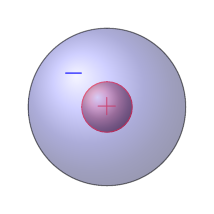
\begin{tikzpicture}
				\node[circle, draw=red, ball color=red!50, inner sep=0.1cm, text=red] (O) at (0,0)
				{$+$};
				\draw[ball color=blue!50, opacity=0.5] (O) circle (1);
				\node[text=blue] at (135:0.6) {$-$};
			\end{tikzpicture}
			\begin{block}{}\centering\scriptsize
				Дипольний момент без зовнішнього поля $p = 0$.
			\end{block}
		\end{column}
		\begin{column}{0.5\linewidth}
			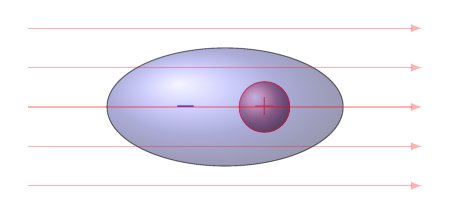
\begin{tikzpicture}[>=latex]
				\node[circle, draw=red, ball color=red!50, inner sep=0.1cm, text=red] (O) at (0,0)
				{$+$};
				\draw[ball color=blue!50, opacity=0.5] ([xshift=-0.5cm]O) ellipse (1.5 and 0.75);
				\node[text=blue] at (180:1) {$-$};

				\foreach \y in {-1,-0.5,...,1}
					{
						\draw[->, red, opacity=0.3] (-3, \y) -- ++(5, 0);
					}
			\end{tikzpicture}
			\begin{block}{}\centering\scriptsize
				Дипольний момент виник під дією зовнішнього поля $p \neq 0$.
			\end{block}
		\end{column}
	\end{columns}
	\begin{block}{} \justifying
		Прикладом неполярних молекул є кисень (\ce{O2}), азот (\ce{N2}), метан (\ce{CH4}) атоми
		інертних газів.
	\end{block}
\end{frame}
% ===========================================================================




% ============================== Слайд ## ===================================
\begin{frame}{Поле точкового диполя}
	\begin{onlyenv}<1>
		\begin{block}{}\justifying
			Диполь називається \alert{точковим}, якщо відстань між його зарядами
			(плече диполя) $\ell$ мала порівняно з відстанню $r$ від диполя до
			точки спостереження: $\ell \ll r$.
		\end{block}

		\begin{columns}
			\begin{column}{0.75\linewidth}
				\begin{block}{}\justifying
					Поле точкового диполя можна знайти за допомогою принципу
					суперпозиції
					та з урахуванням нерівності $\ell \ll r$:
					\begin{equation*}
						\vec{E} = \frac{(-q)\vec{r}_-}{r_-^3} +
						\frac{(+q)\vec{r}_+}{r_+^3}, \quad
						\begin{cases}
							\vec{r}_- =  \vec{r} + \vec{\ell}/2 \\
							\vec{r}_+ =  \vec{r} - \vec{\ell}/2
						\end{cases}.
					\end{equation*}
					\begin{equation*}
						\tcbhighmath{
							\vec{E} = \frac{3(\vec{p}\cdot\vec{r})\vec{r}}{r^5} -
							\frac{\vec{p}}{r^3}.
						}
					\end{equation*}

					Таким чином, напруженість поля точкового диполя зменшується з
					відстанню за законом
					\begin{equation*}
						E \sim 1/{r^3}.
					\end{equation*}
				\end{block}
			\end{column}
			\begin{column}{0.25\linewidth}\centering
				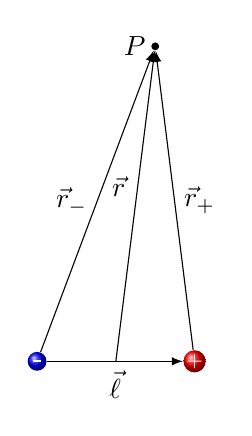
\begin{tikzpicture}[>=latex]
	\node [circle, ball color=blue, inner sep=1.2pt, text=white]
	(qn) at (-1,0) {\tikz\draw[thick] (0,0) -- ++(0.1,0);};

	\node [circle, ball color=red, inner sep=0pt, text=white,
		font=\scriptsize] (qp) at (1,0) {$+$};

	\draw[->] (qn) -- node[below] {$\vec{\ell}$} (qp);

	\node[fill, circle, inner sep=1pt] (P) at  (0.5, 4) {};
	\node[left] at (P) {$P$};

	\draw[->] (0,0) -- node[above left] {$\vec{r}$} (P);

	\draw[->] (qn) -- node[left] {$\vec{r}_-$} (P);
	\draw[->] (qp) -- node[right] {$\vec{r}_+$} (P);
\end{tikzpicture}
			\end{column}
		\end{columns}
	\end{onlyenv}
	\framesubtitle<2>{Виведення}
	\begin{onlyenv}<2>
		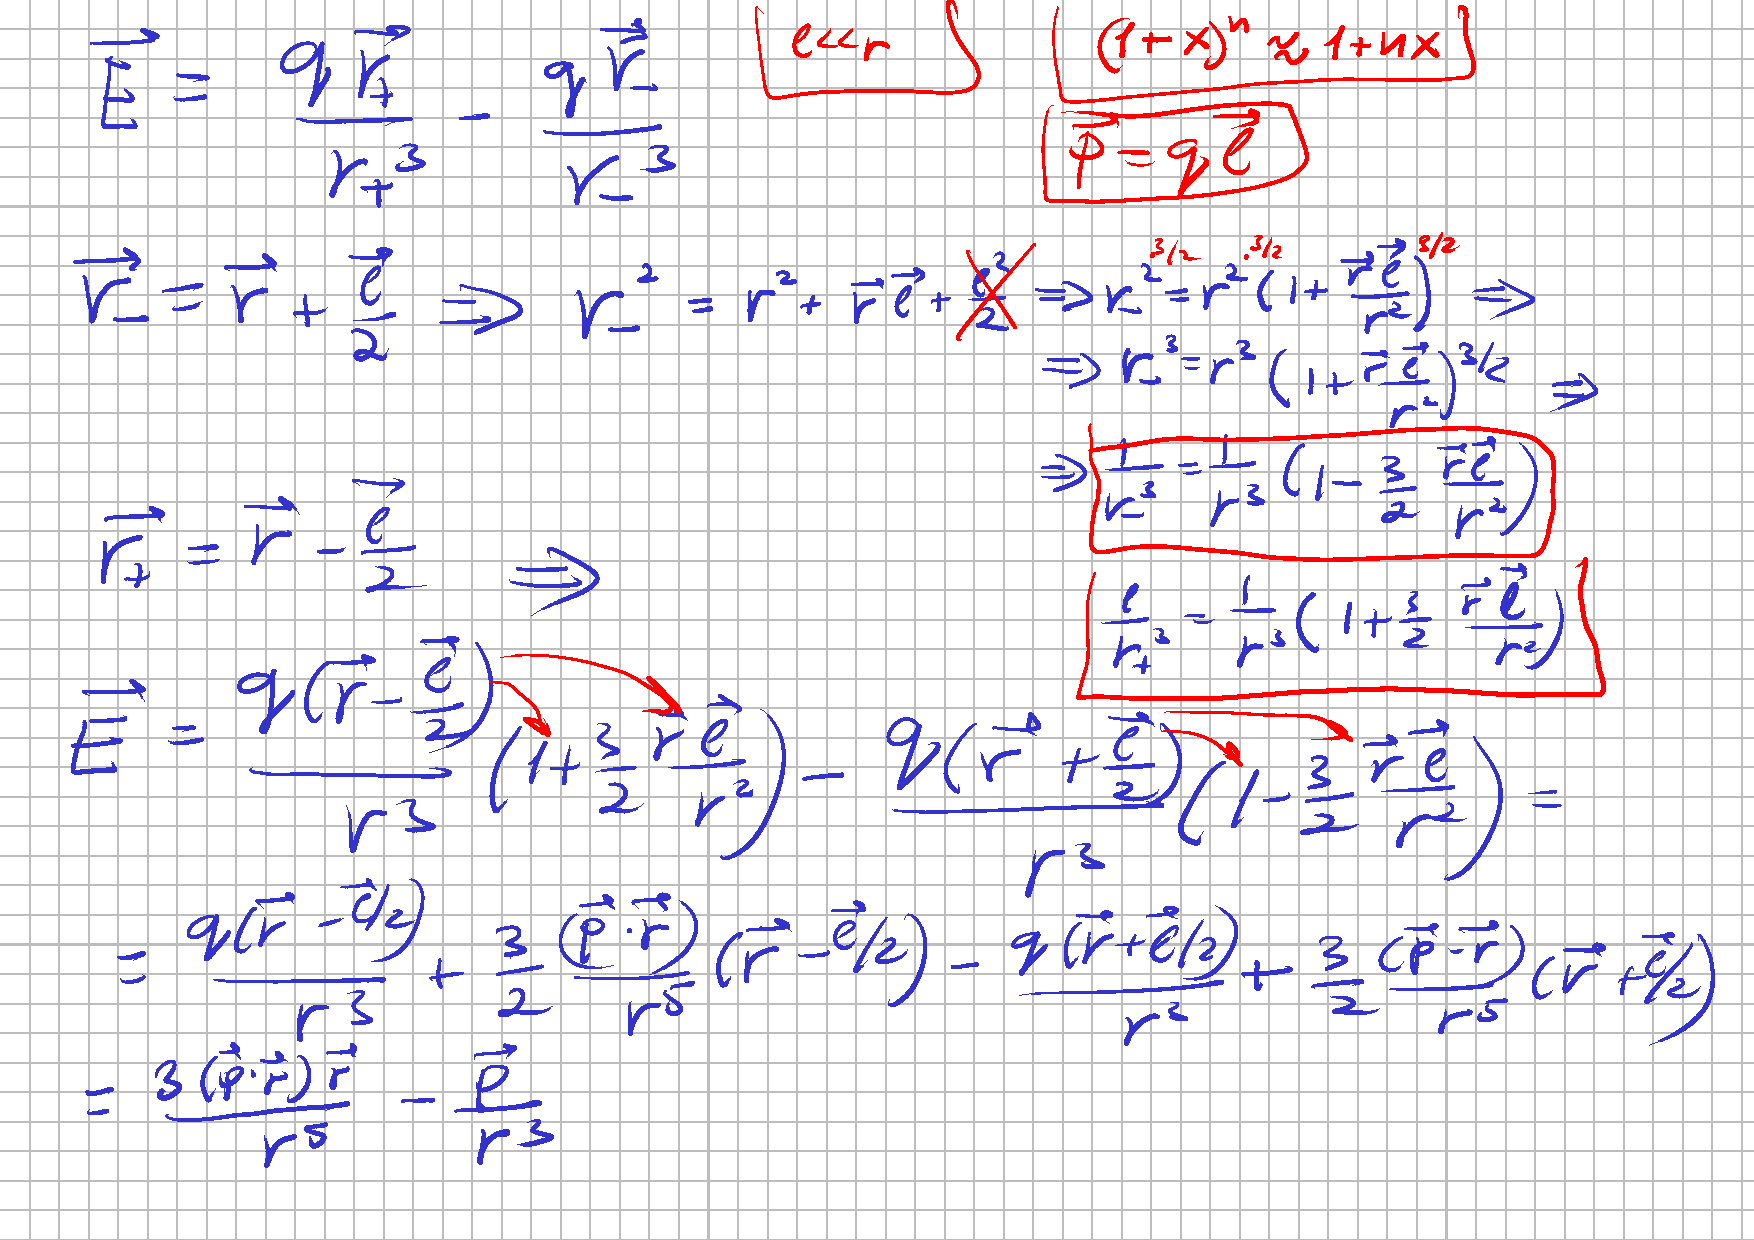
\includegraphics[width=\linewidth]{dipolefield.pdf}
	\end{onlyenv}
\end{frame}
% ===========================================================================



% ============================== Слайд ## ===================================
\begin{frame}{Момент сил, що діє на диполь в однорідному полі}{}
	\begin{center}
		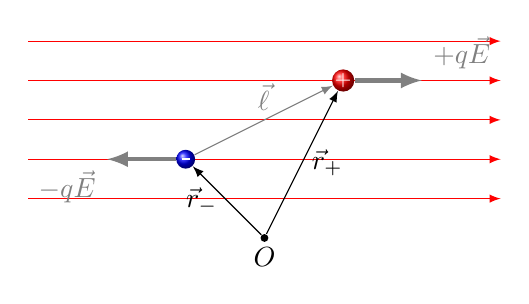
\begin{tikzpicture}[>=latex]
	\foreach \i in {-1,-0.5,...,1} {
			\draw[->, red] (-3, \i) -- ++(6, 0);
		}

	\node [circle, ball color=blue, inner sep=1.2pt, text=white]
	(qn) at (-1,-0.5) {\tikz\draw[thick] (0,0) -- ++(0.1,0);};

	\node [circle, ball color=red, inner sep=0pt, text=white,
		font=\scriptsize] (qp) at (1,0.5) {$+$};


	\draw[->, ultra thick, gray] (qn) -- ++(-1, 0) node[below left]
	{$-q\vec{E}$};

	\draw[->, ultra thick, gray] (qp) -- ++(1, 0) node[above right]
	{$+q\vec{E}$};

	\node[inner sep=1pt, circle, fill] (O) at (0, -1.5) {};
	\node[below] at (O) {$O$};

	\draw[->] (O) -- node[left] {$\vec{r}_-$}(qn);
	\draw[->] (O) -- node[right] {$\vec{r}_+$}(qp);

	\draw[->, gray] (qn) -- node[above] {$\vec{\ell}$} (qp);
\end{tikzpicture}
	\end{center}

	\begin{equation*}
		\tcbhighmath{
			\vec{M} = \left[\vec{p}\times\vec{E}\right].
		}
	\end{equation*}

	\begin{alertblock}{}
		Диполь в електричному полі орієнтується за напрямком поля.
	\end{alertblock}
\end{frame}
% ===========================================================================




% ============================== Слайд ## ===================================
\begin{frame}{Густини електричного заряду}{}
	\begin{columns}
		\begin{column}{0.7\linewidth}\centering
			\begin{block}{}\justifying
				Виділимо елементарний об'єм $dV$. Якщо в цьому об'ємі міститься заряд $dq$, то
				\alert{об'ємною густиною заряду} називається величина:
				\begin{equation*}
					\rho = \frac{dq}{dV}
				\end{equation*}
			\end{block}
		\end{column}
		\begin{column}{0.3\linewidth}\centering
			\begin{tikzpicture}[>=latex,
					charge/.style = {ball color=red!50, font=\scriptsize, inner sep=1pt},
					surface/.style = {draw, opacity=0.5, smooth cycle, tension=.7},
					filled_surface/.style = {red, fill=red!50, smooth cycle, tension=.7},
					>=latex,
					scale=0.7,
					transform shape
				]

				\def\coordinates{
					(-1,0)
					(-0.5,1)
					(0.5,2)
					(2.5,1.5)
					(3,0.5)
					(2,-1.5)
					(0.5,-2)
					(-0.5,-1)
				}

				\begin{scope}[scale=0.7]
					\clip[yshift=2cm] plot[smooth cycle, tension=.7] coordinates \coordinates;
					\draw[yshift=2cm, draw=red, fill=red!40] plot[smooth cycle, tension=.7]
					coordinates \coordinates;
					\draw plot [only marks, mark=+, domain=-1:3, samples=100, mark
					options={color=red}]
					(\x,{rnd*4});
				\end{scope}
				\begin{scope}[shift={(55:2cm)}, line join=round]
					\pgfmathsetmacro{\cubex}{0.2}
					\pgfmathsetmacro{\cubey}{0.2}
					\pgfmathsetmacro{\cubez}{0.2}
					\draw[fill=red] (0,0,0) -- ++(-\cubex,0,0) -- ++(0,-\cubey,0) -- ++(\cubex,0,0)
					-- cycle;
					\draw[fill=red] (0,0,0) -- ++(0,0,-\cubez) -- ++(0,-\cubey,0) -- ++(0,0,\cubez)
					-- cycle;
					\draw[fill=red] (0,0,0) -- ++(-\cubex,0,0) -- ++(0,0,-\cubez) -- ++(\cubex,0,0)
					-- cycle;
				\end{scope}
				\node[font=\scriptsize, anchor=south west, inner sep=1pt, text
					width=2cm,
					align=center, text=blue] (div1) at (2.2,1) {Елемент об'єму \\ $dV$};
				\draw[<-, gray, thick] (55:2cm)
				to[out=45, in = 135] (div1.north west);
			\end{tikzpicture}
		\end{column}
	\end{columns}
	\begin{columns}
		\begin{column}{0.7\linewidth}
			\begin{block}{}\justifying
				Якщо заряд розподілений у тонкому шарі. Виділимо елемент шару
				площею $dS$, що несе заряд $dq$. \alert{Поверхневою густиною} заряду називається
				величина:
				\begin{equation*}
					\sigma = \frac{dq}{dS}
				\end{equation*}
			\end{block}
		\end{column}
		\begin{column}{0.3\linewidth}\centering
			\begin{tikzpicture}[>=latex, every node/.style={font=\scriptsize}, scale=0.7,
					transform shape]
				\draw[fill=red!40, scale=0.7] (0,0) to[bend left] ++(2,1.9)  to[bend left]
				++(2,-2)
				to[bend right] ++(-2, -1)  to[bend right] cycle;
				\coordinate (A) at (1.3, 0.8);
				\draw[fill=red] (A) circle(0.2 and 0.1);
				\node[font=\scriptsize, anchor=south west, inner sep=1pt, text
					width=2.5cm,
					align=center, text=blue] (div1) at (2.5,1) {Елемент поверхні \\ $dS$};
				\draw[<-, gray, thick] (A)
				to[out=45, in = 135] (div1.north west);
			\end{tikzpicture}
		\end{column}
	\end{columns}
	\begin{columns}
		\begin{column}{0.7\linewidth}
			\begin{block}{}\justifying
				\alert{Лінійна густина} --- заряд, що
				припадає на одиницю довжини нитки (зразка, поперечні розміри якого малі
				порівняно з поздовжніми розмірами):
				\begin{equation*}
					\lambda = \frac{dq}{dl}
				\end{equation*}
			\end{block}
		\end{column}
		\begin{column}{0.3\linewidth}
			\begin{tikzpicture}[>=latex, every node/.style={font=\scriptsize}, scale=0.7, transform
					shape]
				\draw[red!40, line width=3pt] plot[domain=0.4:0.8*pi] ({\x}, {sin(\x r)});
				\draw[red, line width=3pt] plot[domain=1:1.4] ({\x}, {sin(\x r)});
				\node[font=\scriptsize, anchor=south west, inner sep=1pt, text width=2.5cm,
					align=center, text=blue] (div1) at (2.2,1) {Елемент довжини \\ $dl$};
				\draw[<-, gray, thick] (1.2, {sin(1.2 r)}) to[out=65, in = 135] (div1.north west);
			\end{tikzpicture}
		\end{column}
	\end{columns}
\end{frame}
% ===========================================================================




% ============================== Слайд ## ===================================
\begin{frame}{Задача}{Поле рівномірно зарядженого диска на осі}
	\begin{exampleblock}{}\justifying
		Нехай є тонкий диск радіуса $R$, поверхнею якого рівномірно розподілено
		заряд $Q$. Знайти електричне поле на осі диска на відстані $z$ від його
		площини.
	\end{exampleblock}
	\begin{center}
		\begin{tikzpicture}[>=latex, every node/.style={font=\scriptsize,inner sep=2pt}, scale=1.5, transform shape]
    \draw[fill=gray!50] (0, 0) circle (1 and 0.3);
    \draw[fill=gray!50] (-1, 0) -- ++(0,-0.1) arc(180:360:1 and 0.3) -- ++(0, 0.1) arc(0:-180:1 and 0.3) ;
    \draw[-stealth] (0,0) -- ++(0, 2) node[left] {$z$};
    \draw[->] (0,0) -- node[above] {$R$} (-50:1 and 0.3);
    \draw[fill=red] (150:0.8 and 0.23) arc(150:210:0.8 and 0.23) -- (210:0.7 and 0.17) arc(210:150:0.7 and 0.17) -- cycle;

    \draw[->] (180:0.75) coordinate (r) -- node[above] {$\vect{r}$} (0, 1.5) node[circle, fill, inner sep=0.25pt] (P) {};
    \node[left] at (P) {$P$};
    \draw[->, red] (P) -- ++({atan(1.5/0.75)}:0.5) node[above] {$d\Efield$};
    \draw [] (P) ++(0,-0.5)  arc(-90:atan(1.5/0.75)-180:0.5) node[anchor=north, pos=0.6] {$\theta$};
    \draw[->] (0 ,0) -- node[below] {$\vect{r}'$} ++(210:0.7 and 0.17);
    \draw[] (0 ,0) -- ++(150:0.7 and 0.17);
    \draw (205:0.25 and 0.08) arc(205:155:0.25 and 0.08) coordinate[pos=0.5] (dphi);
    \node (dphi1) at (-0.25, 0.4) {$d\phi$};
    \draw[-{Latex[length=3pt, open]}, blue] (dphi1.south) to[bend right] (dphi);
    \node (dS) at (-1.25, 0.2) {$\sigma dS$};
    \draw[-{Latex[length=3pt, open]}, blue] (dS) to[bend right] (r);
    \draw[dash pattern={on 1pt off 0.5pt}] (0,0) --++ (0.25, 0);
    \draw[dash pattern={on 1pt off 0.5pt}] (P) -- ++(0.25, 0);
    \draw[<->] (0.15, 1.5) -- node[circle, fill=white, inner sep=1pt] {$z$} (0.15, 0);
\end{tikzpicture}
	\end{center}
\end{frame}
% ===========================================================================





%% --------------------------------------------------------
\section{Теорема Гаусса для електричного поля у вакуумі}
%% --------------------------------------------------------
% ============================== Слайд ## ===================================
\begin{frame}{Чи достатньо цього?}{}
	\begin{alertblock}{}\centering
		Чи достатньо закону Кулона і принципу суперпозиції для визначення
		напруженості електричного поля довільної системи зарядів?
	\end{alertblock}
	\begin{block}{}\justifying
		Для простих випадків \alert{закон Кулона} і \alert{принцип
			суперпозиції} є ефективними \alert{інструментами для обчислення
			електричного поля}. Проте, у випадках із складною геометрією розподілу
		зарядів, ці методи можуть бути недостатньо зручними для аналітичних
		розрахунків. Тому в теорії електричних полів були \alert{введені
			допоміжні концепції та методи}, які \alert{спрощують обчислення і
			аналіз} полів у складних системах, дозволяючи ефективніше вирішувати
		задачі, включаючи аналітичні розв’язки.
	\end{block}

	\begin{exampleblock}{}\justifying\small
		Наприклад, спробуйте обчислити за допомогою закону Кулона і принципу
		суперпозиції напруженість поля всередині рівномірно зарядженої кулі. Вийде
		так, що інтеграли буде практично неможливо вирішити аналітичним методом.
		Чисельно (на комп'ютері), це зробити можна, але чисельні результати не
		можна якісно проаналізувати. Далі вводяться концепції та методи, які
		дадуть змогу зробити це аналітично.
	\end{exampleblock}

	\begin{alertblock}{Концепції --- абетка теорії поля}\justifying
		Потік вектора, потенціал, циркуляція вектора, теореми Гаусса та теорема
		про циркуляцію
	\end{alertblock}
\end{frame}
% ===========================================================================



% ============================== Слайд ## ===================================
\begin{frame}{Потік вектора}{}
	\begin{block}{}\justifying
		Порахуємо об'єм рідини $dV$, що протікає за час $dt$ через поверхню $S$
	\end{block}
	\begin{columns}
		\begin{column}{0.45\linewidth}\centering
			\begin{tikzpicture}[scale=0.8, >=latex, midarrow/.style={%
							postaction={ decorate,
									decoration={ markings, mark=at position .7 with
												{\arrow{stealth}}}}}]

				\foreach \y in {-5,-3,...,5}{
						\draw[blue!50, midarrow, line width=0.5pt] plot[domain=0.5:6] (\x,
						0.2*\y+0*\y*\x^2);
					}
				\draw[->, blue] (2, 0) -- ++(1.5,0) node[right, text=red] {$\vect{v}$};
				\draw[->] (2, 0) -- ++(1,0) node[above right] {$\vect{n}$};
				\draw[red, fill=red!50, opacity=0.5] (2,0) circle (0.5 and 0.85);
				\draw[dashed, thick] (2, 0.85) -- ++(3,0);
				\draw[dashed, thick] (2, -0.85) -- node[below] {$dl$} ++(3,0);
				\draw[dashed, thick] (5,0) circle (0.5 and 0.85);
				\node[opacity=0.3] at (3.2, 0) {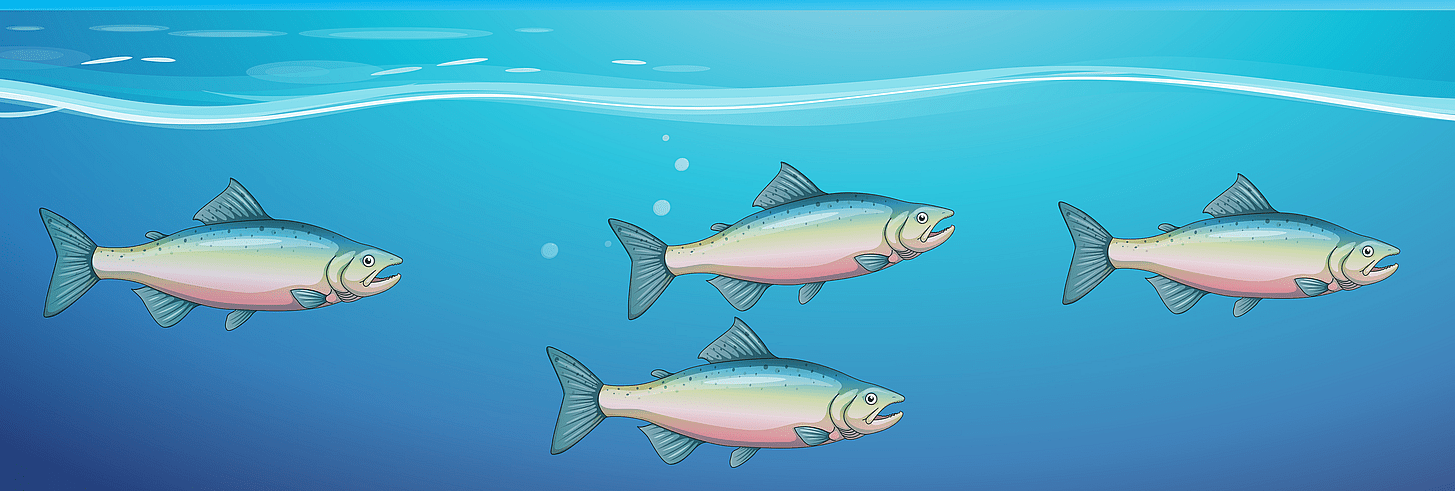
\includegraphics[width=\linewidth]{fishes}};
			\end{tikzpicture}
		\end{column}
		\begin{column}{0.45\linewidth}\centering
			\begin{tikzpicture}[scale=0.8, >=latex, midarrow/.style={%
							postaction={ decorate,
									decoration={ markings, mark=at position .7 with
												{\arrow{stealth}}}}}]

				\foreach \y in {-5,-3,...,5}{
						\draw[blue!50, midarrow, line width=0.5pt] plot[domain=0.5:6] (\x,
						0.2*\y+0*\y*\x^2);
					}
				\draw[->, blue] (2, 0) -- ++(1.5,0) node[right, text=red] {$\vect{v}$};
				\draw[->] (2, 0) -- ++(-45:1) node[above right] {$\vect{n}$};
				\draw[red, fill=red!50, opacity=0.5, rotate around={-45:(2,0)}] (2,0) circle
				(0.5
				and 0.85);
				\draw[dashed, thick] (1.6, 0) ++(45:1) -- ++(3,0);
				\draw[dashed, thick] (2.4, 0) ++(-135:1) -- node[below] {$dl$} ++(3,0);
				\draw[dashed, thick, rotate around={-45:(5,0)}] (5,0) circle (0.5
				and 0.85);
				\node[opacity=0.3] at (3.2, 0) {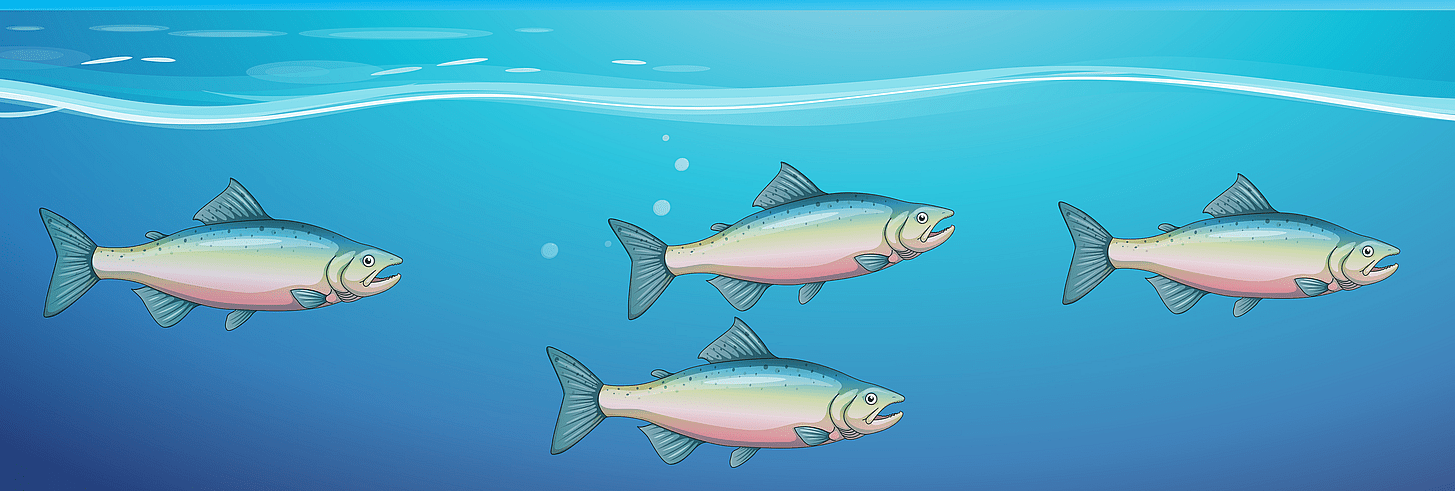
\includegraphics[width=\linewidth]{fishes}};
			\end{tikzpicture}
		\end{column}
	\end{columns}
	\begin{equation*}
		\frac{dV}{dt} = v_n S = \vect{v} \cdot \vect{n}\ S = \vect{v} \cdot \vect{S}, \quad
		\vect{S}
		= \vect{n}S
	\end{equation*}
	\begin{block}{}\justifying
		Об'єм рідини, що протікає за одиницю часу $dV/dt = \Phi$ через поверхню~$S$ ---
		\alert{потік
			вектора швидкості}!
	\end{block}
	\begin{columns}
		\begin{column}{0.35\linewidth}
			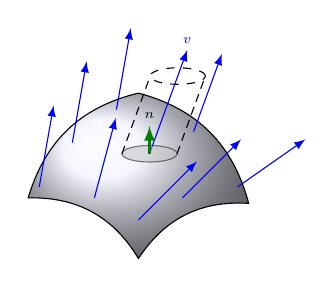
\begin{tikzpicture}[>=latex, every node/.style={font=\scriptsize}, scale=0.7,
					transform shape]
				\draw[ball color=blue!5] (0,0) to[bend left] ++(2,1.9)  to[bend left] ++(2,-2)
				to[bend right]
				++(-2, -1)  to[bend
					right] cycle;
				\draw[->, blue] (0.2, 0.2) -- ++(80:1.5);
				\draw[->, blue] (0.8, 1) -- ++(80:1.5);
				\draw[->, blue] (1.6, 1.6) -- ++(80:1.5);

				\draw[->, blue] (1.2, 0) -- ++(75:1.5);
				\draw[->, blue] (2.2, 0.8) coordinate (A) -- ++(70:2) coordinate (B)
				node[above] {$\vect{v}$};
				\draw[->, blue] (3, 1.2) -- ++(70:1.5);

				\draw[->, blue] (2, -0.4) -- ++(45:1.5);
				\draw[->, blue] (2.8, 0) -- ++(45:1.5);
				\draw[->, blue] (3.8, 0.2) -- ++(35:1.5);

				\draw[fill=gray!50, opacity=0.5] (A) circle(0.5 and 0.15);
				\draw[dashed] (A) ++(70:1.5) circle(0.5 and 0.15);
				\draw[->, green!50!black, thick] (A) -- ++(90:0.5) node[above, text=black]
				{$\vect{n}$};
				\draw[densely dashed] (A) ++(180:0.5) -- ++(70:1.5);
				\draw[densely dashed] (A) ++(0:0.5) -- ++(70:1.5);
			\end{tikzpicture}
		\end{column}
		\begin{column}{0.6\linewidth}
			\begin{block}{}\justifying
				Для довільної (не обов'язково плоскої) поверхні потік через елементарну
				площадку $d\Phi = v_n dS = \vect{v}\cdot d\vect{S}$. А через всю поверхню~$S$:
				\begin{equation*}
					\Phi = \iint\limits_S \vec{v}\cdot d\vec{S}
				\end{equation*}
			\end{block}

		\end{column}
	\end{columns}
\end{frame}
% ===========================================================================






% ============================== Слайд ## ===================================
\begin{frame}{Потік вектора $\Efield$}{}
	\begin{columns}
		\begin{column}{0.5\linewidth}
			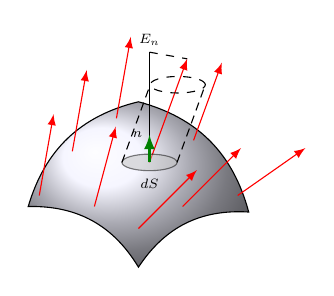
\begin{tikzpicture}[>=latex, every node/.style={font=\scriptsize}, scale=0.7,
					transform shape]
				\draw[ball color=blue!5] (0,0) to[bend left] ++(2,1.9)  to[bend left] ++(2,-2)
				to[bend right]
				++(-2, -1)  to[bend
					right] cycle;
				\draw[->, red] (0.2, 0.2) -- ++(80:1.5);
				\draw[->, red] (0.8, 1) -- ++(80:1.5);
				\draw[->, red] (1.6, 1.6) -- ++(80:1.5);

				\draw[->, red] (1.2, 0) -- ++(75:1.5);
				\draw[->, red] (2.2, 0.8) coordinate (A) -- ++(70:2) coordinate (B)
				node[above] {$\Efield$};
				\draw[->, red] (3, 1.2) -- ++(70:1.5);

				\draw[->, red] (2, -0.4) -- ++(45:1.5);
				\draw[->, red] (2.8, 0) -- ++(45:1.5);
				\draw[->, red] (3.8, 0.2) -- ++(35:1.5);

				\draw[fill=gray!50, opacity=0.5] (A) circle(0.5 and 0.15);
				\draw[dashed] (A) ++(70:1.5) circle(0.5 and 0.15);
				\draw[] (A) -- ++(90:2) coordinate (C) node[above, text=black]
					{$E_n$};
				\draw[->, green!50!black, thick] (A) -- ++(90:0.5) node[left, text=black]
				{$\vect{n}$};
				\draw[densely dashed] (A) ++(180:0.5) -- ++(70:1.5);
				\draw[densely dashed] (A) ++(0:0.5) -- ++(70:1.5);
				\draw[dashed] (C) -- (B);
				\node[below=5pt] at (A) {$dS$};
			\end{tikzpicture}

		\end{column}
		\begin{column}{0.5\linewidth}\centering
			\begin{tikzpicture}[scale=0.5, >=latex, midarrow/.style={%
							postaction={ decorate,
									decoration={ markings, mark=at position .7 with
												{\arrow{stealth}}}}}]

				\foreach \y in {-4,...,4}{
						\draw[red!50, midarrow, line width=0.5pt] plot[domain=0.5:6] (\x,
						0.2*\y+0.01*\y*\x^2);
					}

				\node[] at (4,-1.6)
				{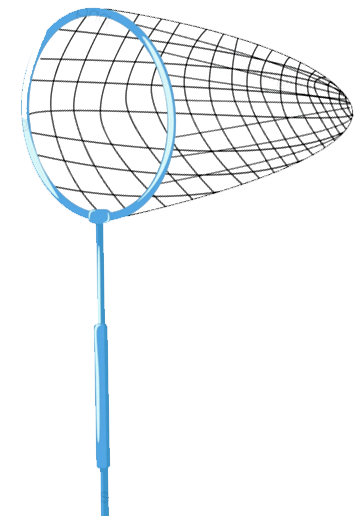
\includegraphics[width=0.4\linewidth]{pictures/butterflynet}};
			\end{tikzpicture}
		\end{column}
	\end{columns}
	\begin{block}{}\centering\justifying
		Потік вектора $\Efield$ через елементарну площадку $dS$:
		\begin{equation*}
			d\Phi = E_n dS = \Efield\cdot d\vect{S}.
		\end{equation*}
	\end{block}
	\begin{block}{}\justifying
		Інтеграл
		\begin{equation*}
			\Phi = 	\iint\limits_S \vec{E}\cdot d\vec{S} = \iint\limits_S E_n\ dS
		\end{equation*}
		називають \alert{потоком вектора напруженості електричного поля} $\vec{E}$ через поверхню
		$S$, хоча з цим поняттям і не пов'язана жодна реальна течія.
	\end{block}
\end{frame}
% ===========================================================================




% ============================== Слайд ## ===================================
\begin{frame}{Теорема Гаусса}{}
	\begin{block}{Теорема Гаусса}\justifying
		Потік вектора напруженості електричного поля через довільно
		обрану замкнуту поверхню пропорційний електричному заряду, що знаходиться
		всередині цієї поверхні:

	\end{block}
	\begin{columns}
		\begin{column}{0.5\linewidth}
			\begin{equation*}
				\tcbhighmath{
					\oiint\limits_{\tikzmarknode{S}{S}} \vec{E}\cdot
					d\vec{S} =
					4\pi \iiint\limits_{\tikzmarknode{V}{V}} \rho dV.
				}
			\end{equation*}
			\tikz[remember picture, overlay]{\draw[-latex,red] (V.south west)
				to[bend left] (S.south east);}
		\end{column}
		\begin{column}{0.5\linewidth}\centering
			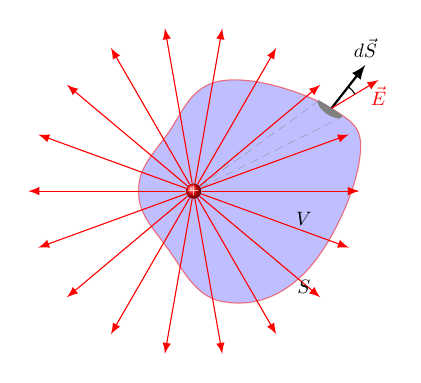
\begin{tikzpicture}[surface/.pic = {
				\fill[blue!50, draw=red, opacity=0.5]  plot[smooth
						cycle, tension=.7]
				coordinates {
						(-1,0)
						(-0.5,1)
						(0.5,2)
						(2.5,1.5)
						(3,0.5)
						(2,-1.5)
						(0.5,-2)
						(-0.5,-1)
					};
			},
		>=latex,
		scale=0.7,
		transform shape
	]
	\pic[] at (0,0)  {surface};

	\node [circle, ball color=red, inner sep=0pt, text=white,
		font=\scriptsize] (qp) at (0,0) {$+$};

	\foreach \i in {0,20,...,360} {
			\draw[->, red] (qp) -- (\i:3);
		}
	\draw[gray, ultra thin, densely dashed] (qp) -- (35.8:2.8)
	coordinate
	(A);
	\draw[gray, ultra thin, densely dashed] (qp) -- (26.5:3)
	coordinate (B);

	\coordinate (S) at (2.5,1.5);

	\draw[->, thick] (S) -- ++(52:1) node[above] {$d\vec{S}$};
	\fill[rotate around={-35:(S)}, gray, draw] (A) arc[start
			angle = -180,
			delta
			angle=190, x radius= 0.25cm, y radius=0.1cm] -- (S) -- (A) --
	cycle;

	%             \draw[->, red] (qp) -- (31:4);
	\draw[->, red] (S) -- ++(31:1) node[below] {$\vec{E}$};

	\draw (S)  ++(52:0.5) arc[radius = 0.5cm, start angle=52, end
			angle=31];

	\node[below] at (2,-1.5) {$S$};
	\node[] at (2, -0.5) {$V$};
\end{tikzpicture}
		\end{column}
	\end{columns}

	\begin{block}{}\justifying\small
		\alert{Для розрахунку електричних полів системи зарядів теореми Гаусса
			недостатньо, бо вона є скалярним співвідношенням}, чого
		замало для визначення трьох невідомих --- складових $E_x$, $E_y$, $E_z$
		вектора $\vec{E}$. \alert{Необхідна відома симетрія задачі}, щоб остання
		звелася до розв'язання одного скалярного рівняння.
	\end{block}

\end{frame}
% ===========================================================================


% ============================== Слайд ## ===================================
\begin{frame}{Приклади застосування теореми Гаусса}{}
	\begin{enumerate}
		\item Поле рівномірно зарядженої площини.
		\item Поле рівномірно різнойменно заряджених площини.
		\item Поле рівномірно зарядженої нитки.
		\item Поле рівномірно зарядженої сфери.
		\item Поле рівномірно зарядженої кулі.
		\item Поле в порожнині рівномірно зарядженої кулі.
	\end{enumerate}
\end{frame}
% ===========================================================================

% ============================== Слайд ## ===================================
\begin{frame}{Поле рівномірно зарядженої площини}{}
	\begin{columns}
		\begin{column}{0.5\linewidth}\centering
			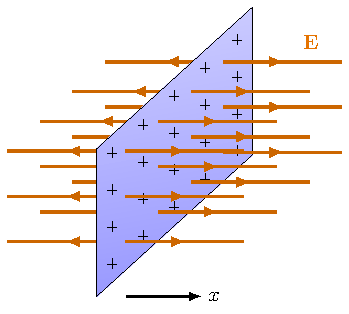
\includegraphics[scale=1,page=1]{tikz/GaussExamples.pdf}
		\end{column}
		\begin{column}{0.5\linewidth}\centering
			\includegraphics[scale=1,page=2]{tikz/GaussExamples.pdf}
		\end{column}
	\end{columns}

	\begin{equation*}
		\tcbhighmath{
			E = 2\pi\sigma.
		}
	\end{equation*}

\end{frame}
% ===========================================================================



% ============================== Слайд ## ===================================
\begin{frame}{Поле рівномірно зарядженої кулі}{}
	\begin{onlyenv}<1>
		\begin{columns}
			\begin{column}{0.5\linewidth}\centering
				\includegraphics[scale=1,page=5]{tikz/GaussExamples.pdf}
			\end{column}
			\begin{column}{0.5\linewidth}\centering
				\includegraphics[scale=1,page=4]{tikz/GaussExamples.pdf}
			\end{column}
		\end{columns}
	\end{onlyenv}
	\begin{onlyenv}<2>
		\begin{equation*}
			{E} =
			\begin{cases}
				\dfrac{4\pi}{3}\rho r = \dfrac{Q}{R^3} r, \quad r < R, \\
				\dfrac{Q}{r^2}, \quad r > R.
			\end{cases}
		\end{equation*}

		\begin{center}
			\begin{tikzpicture}
	\begin{axis}[axis lines=middle,
			xtick=\empty,
			ytick=\empty,
			extra x ticks={1},
			extra x tick labels={$R$},
			extra y ticks={1},
			extra y tick labels={$\frac{Q}{R^2}$},
			height=0.5\linewidth,
			width=\linewidth,
			ymax=1.3,
			xlabel=$r$,
			xlabel style={below right},
			ylabel=$E$,
			ylabel style={above left},
		]
		\addplot[domain=0:1, red, thick] {x};
		\addplot[domain=1:3, red, thick] {1/x^2};
		\draw[dashed] (axis cs:1,0) -- (axis cs:1,1);
		\draw[dashed] (axis cs:1,1) -- (axis cs:0,1);
	\end{axis}
\end{tikzpicture}
		\end{center}

	\end{onlyenv}
\end{frame}
% ===========================================================================


% ============================== Слайд ## ===================================
\begin{frame}{Теорема Гаусса в диференціальній формі}{Виведення}
	\begin{onlyenv}<1>
		\begin{columns}
			\begin{column}{0.6\linewidth}\justifying\small
				Виділимо в просторі нескінченно малий прямокутний паралелепіпед зі
				сторонами $dx$, $dy$, $dz$, що паралельні до координатних осей. На
				грані $1$ зовнішня нормаль спрямована у від'ємний бік осі $y$.
				Тому потік вектора $\vec{E}$ через цю грань буде $-E_y(y) dx dz$.
				На протилежній грані $2$, навпаки, напрямок зовнішньої нормалі
				збігається з позитивним напрямком осі $y$, і для потоку через цю
				грань слід писати $E_y(y + dy) dx dz$. Сума обох потоків буде:
				\begin{equation*}
					\left[E_y(y + dy) - E_y(y) \right] dxdz = \left( \frac{\partial
						E_y}{\partial y} dy\right) dxdz = \frac{\partial
						E_y}{\partial y} dV.
				\end{equation*}
			\end{column}
			\begin{column}{0.4\linewidth}\centering
				\begin{tikzpicture}[>=latex, every node/.style={font=\scriptsize}]

    \draw[midarrow, red!40] (1.24,0) to[bend left] ++(75:3);
    \draw[midarrow, red!40] (1.6,0) to[bend left=20pt] ++(70:3);
    \draw[midarrow, red!40] (1.86,0) to[bend left=20pt] ++(55:3);

	\draw[->] (0.5,0.5) -- ++(3, 0) node[below] {$y$};
	\draw[->] (0.5,0.5) -- ++(0, 1) node[above] {$z$};
	\draw[->] (0.5,0.5) -- ++(-135:0.75) node[below] {$x$};

	\draw[green!50!black, thick] (1,2) coordinate (A)
	-- ++(1.5, 0) coordinate (B)
	--   ++(0,-1) coordinate (C)
	-- node[below] {$dy$} ++(-1.5, 0) coordinate (D)
	-- node[left] {$dz$} cycle;

	\path (1.5,2.5) coordinate (A1)
	-- ++(1.5, 0) coordinate (B1)
	-- ++(0,-1) coordinate (C1)
	-- ++(-1.5, 0) coordinate (D1)
	-- cycle;

	\draw[green!50!black, thick] [solid] (A1) --  (B1) -- (C1);
	\draw[green!50!black, thick] [dashed] (C1) -- (D1) -- (A1);

	\draw[green!50!black, thick] (A) -- (A1) (B) -- (B1) (C) -- node[right] {$dx$} (C1);
	\draw[dashed, green!50!black, thick] (D) --(D1);

    \coordinate (E1) at (1.25, 1.75);
    \draw[->, red] (E1) -- ++(65:1.5) coordinate (e1) node[above] {$\Efield(\vect{r})$};
    \draw[red] (E1) -- ++(0:{1.5*cos(65)}) coordinate (e1s) node[right] {$E_y(y)$};
    \draw[dashed] (e1) -- (e1s);
	\draw[->, thick] (E1) node[above, font=\scriptsize] {$1$}  -- ++(-0.5, 0) node[above]
	{$\vec{n}$};

    \coordinate (E2) at ({1.25 + 1.5}, 1.75);
    \draw[->, red] (E2) -- ++(45:1) coordinate (e2) node[above] {$\Efield(\vect{r} + d
    \vect{r})$};
    \draw[red] (E2) -- ++(0:{1*cos(45)}) coordinate (e2s) node[anchor=150, inner sep=1pt]
    {$E_y(y + dy)$};
    \draw[dashed] (e2) -- (e2s);
	\draw[->, thick] (E2) node[above, font=\scriptsize] {$2$} -- ++(+0.5, 0) node[above]
	{$\vec{n}$};

\end{tikzpicture}
			\end{column}
		\end{columns}
	\end{onlyenv}
	\begin{onlyenv}<1-2>
		\begin{block}{}
			Аналогічно знайдуться потоки через дві пари інших граней. Повний потік
			через усю поверхню паралелепіпеда:
			\begin{equation*}
				d\Phi = \left( \frac{\partial E_x}{\partial x} + \frac{\partial
					E_y}{\partial y} + \frac{\partial E_z}{\partial z} \right)  dV =
				\divg\vec{E}\ dV.
			\end{equation*}
		\end{block}
	\end{onlyenv}
	\begin{onlyenv}<2>
		За теоремою Гаусса той самий потік дорівнює $4\pi\rho dV$. Прирівнюючи обидва
		вирази, отримаємо
		\begin{equation*}
			\Div\Efield = \tcbhighmath{
				\divg\Efield = 4\pi\rho.
			}
		\end{equation*}
		\begin{block}{}\justifying
			Величина $\divg\Efield$ (або ще позначається як $\Div\Efield$)
			називається дивергенцією вектора $\Efield$.
			\begin{equation*}
				(\Div\Efield = )\ \divg\Efield = \frac{\partial
					E_x}{\partial
					x} +
				\frac{\partial
					E_y}{\partial y} + \frac{\partial E_z}{\partial z}.
			\end{equation*}
		\end{block}
	\end{onlyenv}
\end{frame}
% ===========================================================================


% ============================== Слайд ## ===================================
\begin{frame}{Дивергенція вектора}{}\small
	\begin{alertblock}{}\centering
		Дивергенція вектора --- скалярна величина!
	\end{alertblock}

	% ============================== Слайд ##
	%===================================
	\begin{block}{Означення дивергенції}
		\begin{equation*}
			\Div\Efield = \lim\limits_{V \to 0} \left(  \frac1{V} \oint\limits_S
			\Efield\cdot d\vec{S} \right)
		\end{equation*}
	\end{block}
	% ===========================================================================

	\begin{block}{Векторний оператор <<набла>>}
		\begin{equation*}
			\vect{\nabla} = \vect{e}_x \frac{\partial}{\partial x} +
			\vect{e}_y \frac{\partial}{\partial y} + \vect{e}_z
			\frac{\partial}{\partial z}, \quad \text{декартова система}.
		\end{equation*}
	\end{block}

	\begin{block}{Дивергенція вектора в різних системах}
		\begin{align*}
			\divg\vect{A} & = \frac{\partial A_x}{\partial x}  +
			\frac{\partial A_y}{\partial y} + \frac{\partial A_z}{\partial},
			\quad \text{декартова система
			координат}                                                        \\
			\divg\vect{A} & = \frac{1}{\rho}\frac{\partial \left(\rho A_{\rho
				}\right)}{\partial \rho }+\frac{1}{\rho }\frac{\partial A_{\varphi
					} }{\partial \varphi }+\frac{\partial A_{z}}{\partial z}, \quad
			\text{циліндрична система
			координат}                                                        \\
			\divg\vect{A} &
			=\frac{1}{r^2}\frac{\partial \left(r^2A_r\right)}{\partial r} +
			\frac{1}{r\sin \theta }\frac{\partial}{\partial \theta
			}\left(A_{\theta }\sin \theta \right) +
			\frac{1}{r\sin\theta}\frac{\partial A_{\varphi}}{\partial \varphi
			}, \quad \text{сферична система координат}
		\end{align*}
	\end{block}
\end{frame}
% ===========================================================================

% ============================== Слайд ## ===================================
\begin{frame}{Теорема Гаусса в диференціальній формі}{Приклади}
	\begin{equation*}
		\tcbhighmath{
			\divg\Efield = 4\pi\rho.
		}
	\end{equation*}

	\begin{overprint}
		\onslide<1>
		\begin{block}{}\justifying
			У диференціальній формі теорема Гаусса є \alert{локальною теоремою}:
			дивергенція поля $\Efield$ у даній точці залежить тільки від густини
			електричного заряду $\rho$ у тій самій точці і більше ні від чого.
			\begin{center}
				\begin{tikzpicture}[>=latex,
    charge/.style = {ball color=red!50, font=\scriptsize, inner sep=1pt},
    surface/.style = {draw, opacity=0.5, smooth cycle, tension=.7},
    filled_surface/.style = {red, fill=red!50, smooth cycle, tension=.7},
    >=latex,
    scale=0.7,
    transform shape
]

\def\coordinates{
    (-1,0)
    (-0.5,1)
    (0.5,2)
    (2.5,1.5)
    (3,0.5)
    (2,-1.5)
    (0.5,-2)
    (-0.5,-1)
}

\begin{scope}
    \clip[yshift=2cm] plot[smooth cycle, tension=.7] coordinates \coordinates;
    \draw[yshift=2cm, draw=red, fill=red!40] plot[smooth cycle, tension=.7]
    coordinates \coordinates;
    \draw plot [only marks, mark=+, domain=-1:3, samples=100, mark
    options={color=red}]
    (\x,{rnd*4});

\end{scope}
    \node[font=\scriptsize, anchor=south west, inner sep=1pt, text
        width=2cm,
    align=center, text=blue] (div0) at (180:4) {В цій точці \\
    $\Div\Efield = 0$ \\ ($\rho = 0$)};
    \draw[<-, gray, thick] (-0.75,0.5) node[inner sep=1pt, circle, fill] {}
    to[out=195, in = 60] (div0.north);


    \node[font=\scriptsize, anchor=south west, inner sep=1pt, text
        width=2cm,
    align=center, text=blue] (div1) at (45:4) {В цій точці \\
    $\Div\Efield = 4\pi\rho$ \\ ($\rho \neq 0$)};
    \draw[<-, gray, thick] (45:2) node[inner sep=1pt, circle, fill] {}
    to[out=45, in = -135] (div1.south);


\end{tikzpicture}

			\end{center}
		\end{block}


		\onslide<2>
		\begin{center}
			\begin{tikzpicture}[>=latex,
		surface/.pic = {
				\draw[opacity=0.5]  plot[smooth
						cycle, tension=.7]
				coordinates {
						(-1,0)
						(-0.5,1)
						(0.5,2)
						(2.5,1.5)
						(3,0.5)
						(2,-1.5)
						(0.5,-2)
						(-0.5,-1)
					};
			},
		>=latex,
		scale=0.7,
		transform shape
	]


	\begin{scope}
		\foreach \i in {20,40,...,360}
			{
				\draw[->, red!50] (0,0)  ++(\i:0.1) -- ++(\i:2);
			}

		\node[font=\scriptsize, anchor=south west, inner sep=1pt, text
		width=2cm,
			align=center, text=blue] (divi) at (15:2.1) {В цій точці \\
			$\Div\Efield =
				\infty$ \\ (виток поля)};
		\draw[<-, gray, thick] (0,0) to[out=45, in = -135] (divi.south west);
		\coordinate (zd) at (120:1.8);
		\pic[gray, scale=0.1] at  (zd)  {surface};
		\node[font=\scriptsize, anchor=south west, inner sep=1pt, text
		width=2cm,
			align=center, text=blue] (div0) at (180:4) {В цій точці \\
			$\Div\Efield =
				0$ \\ (витоків нема)};
		\draw[<-, gray, thick] (zd) to[out=195, in = 45] (div0.north);
	\end{scope}

	\begin{scope}[xshift=7cm,
			decoration={
					markings,
					mark=at position 0.5 with {\arrow{<}}}
		]
		\foreach \i in {20,40,...,360}
			{
				\draw[postaction={decorate}, blue!50] (0,0)  ++(\i:0.1) --
				++(\i:2);
			}

		\node[font=\scriptsize, anchor=south west, inner sep=1pt, text
		width=2cm,
			align=center, text=red] (divi) at (10:2.1) {В цій точці \\
			$\Div\Efield =
				-\infty$ \\ (стік поля)};
		\draw[<-, gray, thick] (0,0) to[out=45, in = -135] (divi.south west);
		\coordinate (zd) at (120:1.8);
		\pic[gray, scale=0.1] at  (zd)  {surface};
		\node[font=\scriptsize, anchor=south west, inner sep=1pt, text
		width=2cm,
			align=center, text=red] (div0) at (210:4) {В цій точці \\
			$\Div\Efield =
				0$ \\ (стоків нема)};
		\draw[<-, gray, thick] (zd) to[out=195, in = 45] (div0.north);
	\end{scope}

\end{tikzpicture}

		\end{center}
		\begin{block}{}\justifying
			У тих точках поля, де дивергенція поля $\Efield$ \alert{більша нуля}, ми
			маємо \alert{джерела поля} (позитивні заряди), а в тих точках, де вона
			\alert{менше нуля}, --- стоки (негативні заряди). Лінії вектора $\Efield$
			виходять із витоків поля, а в місцях стоків вони закінчуються.
		\end{block}
	\end{overprint}

\end{frame}
% ===========================================================================





% ============================== Слайд ## ===================================
\begin{frame}{Задачі}{}
	\begin{exampleblock}{Задача 1}\justifying
		Знайти дивергенцію вектора напруженості поля точкового заряду
		\begin{equation*}
			\Efield = \frac{q}{r^2} \frac{\vect{r}}{r}
		\end{equation*}
		в області $r >0$ шляхом взяття часткових похідних.
		Спробуйте взяти дивергенцію в декартових та сферичних координатах.
	\end{exampleblock}
\end{frame}
% ===========================================================================




%% --------------------------------------------------------
\section{Потенціал}
%% --------------------------------------------------------





% ============================== Слайд ## ===================================
\begin{frame}{Потенціал електричного поля}{}
	\begin{columns}
		\begin{column}{0.7\linewidth}\justifying
			Робота сил поля під час переміщення заряду q з точки $1$ у точку $2$
			дорівнює:
			\begin{equation*}
				A = \int\limits_{(1)}^{(2)} q\Efield(r) d\vec{r} =
				qQ\left(\frac1{r_1} - \frac1{r_2}\right).
			\end{equation*}

		\end{column}
		\begin{column}{0.3\linewidth}\centering
			\begin{tikzpicture}[>=latex, scale=1.3]
	\tikzset{
		draw tangents/.style={decorate,decoration={
						markings,mark=between positions 0 and
						1 step
						.5 with
							{\draw[-latex,black,thin] (0,0) --
								(0.3cm,0)
								node[above] {$\vec{dr}$};},
					}
			}
	}

	\node[circle, fill, inner sep= 1pt] (1) at (-1,1) {};
	\node[circle, fill, inner sep= 1pt] (2) at (1,1) {};
	\draw [green!60!black, thick , postaction=draw tangents] (1)
	..  controls
            (85:1.75) and
            (50:0.5) .. (2);
	\node [circle, ball color=red, inner sep=0pt, text=white,
		font=\scriptsize] (Q) at (0,0) {$+$};

	\node[below=5pt] at (Q) {$Q$};
	\draw[->] (Q) -- node[left] {$\vec{r}_1$} (1);
	\draw[->] (Q) -- node[right] {$\vec{r}_2$} (2);
	\draw[->, red] (Q) -- ++(90:2) node[above] {$\vec{E}$};
	\node[below] at (1) {$1$};
	\node[below] at (2) {$2$};
\end{tikzpicture}
		\end{column}
	\end{columns}
	\begin{overprint}
		\onslide<1>
		\begin{block}{}\justifying
			Ця \alert{робота не залежить від траєкторії}, що з'єднує початкову
			і кінцеву точки. Отже, поле точкового заряду ---
			\alert{консервативне} і можна ввести \alert{потенціальну $U$
				енергію} заряду $q$ у цьому полі: робота сил поля на шляху $1 \to
				2$ дорівнює зменшенню потенціальної енергії заряду $q$:
			\begin{equation*}
				A = U_1 - U_2 = - \Delta U,
			\end{equation*}
			де $ U = \frac{qQ}{r} = q \left( \frac{Q}{r} \right)  = q\phi$, а
			$\phi$
			--- називається \alert{потенціалом електричного поля}.
		\end{block}
		\onslide<2>
		\begin{block}{}\justifying
			Робота сил електростатичного поля під час переміщення заряду $q$
			довільним шляхом із початкової точки $1$ у кінцеву точку $2$
			визначається через \alert{різницю потенціалів $\Delta\phi$}:
			\begin{equation*}
				A = q(\phi_1 - \phi_2) = - q\Delta\phi,
			\end{equation*}
		\end{block}
\begin{alertblock}{}\justifying
    Зазвичай сама величина потенціалу визначається з точністю до деякої адитивної константи, як і сама потенціальна енергія. Можна вибрати якусь реперну
    точку $\vect{r}_0$, в якій покласти потенціал $\phi(\vect{r}_0) = 0$. Зазвичай, таку точку вибирають на нескінченності.
\end{alertblock}
	\end{overprint}
\end{frame}
% ===========================================================================




% ============================== Слайд ## ===================================
\begin{frame}{Циркуляція вектора $\Efield$}
	\begin{columns}
		\begin{column}{0.25\linewidth}\centering
			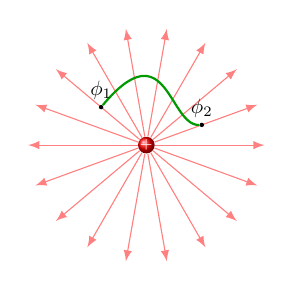
\begin{tikzpicture}[scale=0.75, transform shape, >=latex]
				\node [circle, ball color=red, inner sep=0pt, text=white,
					font=\scriptsize] (qp) at (0,0) {$+$};
				\foreach \i in {20,40,...,360}
					{
						\draw[->, red!50] (qp) -- ++(\i:2);
					}
				\node[circle, inner sep=0.75pt, fill] (1) at (140:1) {};
				\node[circle, inner sep=0.75pt, fill] (2) at (20:1) {};
				\draw [green!60!black, thick] (1) node[above, text=black] {$\phi_1$}  ..  controls
				(80:2) and
				(40:0.5) .. (2) node[above, text=black] {$\phi_2$};
			\end{tikzpicture}
		\end{column}
		\begin{column}{0.75\linewidth}
			\begin{block}{}\justifying
				Різницю потенціалів поля між точками $1$ і $2$ можна виразити через
				напруженість:
				\begin{equation*}
					\int\limits_{(1)}^{(2)} \Efield\cdot d\vect{r} = \phi_1 - \phi_2 = -\Delta\phi.
				\end{equation*}
			\end{block}
		\end{column}
	\end{columns}
	\begin{columns}
		\begin{column}{0.25\linewidth}\centering
			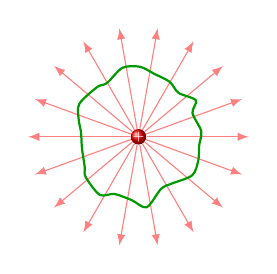
\begin{tikzpicture}[scale=0.7, transform shape,>=latex]
				\node [circle, ball color=red, inner sep=0pt, text=white,
					font=\scriptsize] (qp) at (0,0) {$+$};
				\foreach \i in {20,40,...,360}
					{
						\draw[->, red!50] (qp) -- ++(\i:2);
					}
				% distrorted sphere
				\pgfmathsetseed{2}
				\draw[green!60!black, thick] plot[domain=45:395,smooth cycle]
				(\x:{1+rnd*0.3});
			\end{tikzpicture}
		\end{column}
		\begin{column}{0.75\linewidth}
			\begin{block}{}\justifying
				Оскільки робота поля над зарядом не залежить від форми траєкторії ---
				то для \alert{довільної замкненої траєкторії $L$} маємо
				\begin{equation*}
					\tcbhighmath{
						\oint\limits_L \Efield\cdot d\vect{r}
						% \oint\limits_L \left( E_x dx + 	E_ydy + E_zdz \right)
						= 0
					}
				\end{equation*}
				Цей інтеграл називається \alert{циркуляцією вектора $\Efield$ по
					контуру $L$}, а рівність називається \alert{теоремою про
					циркуляцію в інтегральній формі}.
			\end{block}
		\end{column}
	\end{columns}



\end{frame}
% ===========================================================================


% ============================== Слайд ## ===================================
\begin{frame}{Приклади}
	\begin{exampleblock}{}\centering
		Які конфігурації електростатичного поля можливі?
	\end{exampleblock}
	\begin{columns}
		\begin{column}{0.5\linewidth}\centering
			\begin{tikzpicture}[>=latex, decoration={
							markings, mark=at position 0.5 with
								{\arrow{>}}}]
				\foreach \i in {1,...,8} { \draw[postaction={decorate},
							red, smooth] (0, {1.2^\i-1.2}) -- ++(4, 0); }
				\begin{scope}[visible on=<2>]
					\coordinate (S) at (1,2.6);
					\draw[postaction={decorate}, green!60!black] (S) -- node[above] {$1$} ++(2,0)
					coordinate (1);
					\draw[postaction={decorate}, green!60!black] (1) -- node[right ] {$2$}
					++(0,-1.8)
					coordinate (2);
					\draw[postaction={decorate}, green!60!black] (2) -- node[below] {$3$} ++(-2,0)
					coordinate (3);
					\draw[postaction={decorate}, green!60!black] (3) -- node[left] {$4$} (S);
				\end{scope}
			\end{tikzpicture}
			\begin{block}{}<2>\small
				\begin{multline*}
					\oint_L \Efield\cdot d\vect{r} = \\ E_1 \ell +   \cancelto{0}{\int_2\Efield\cdot
						d\vect{r}}
					-  E_3 \ell + \cancelto{0}{\int_4\Efield\cdot \vect{r}}
					= (E_1 - E_3) \ell \neq 0, \\
					E_1 < E_3
				\end{multline*}
			\end{block}
		\end{column}
		\begin{column}{0.5\linewidth}\centering
			\begin{tikzpicture}[>=latex, decoration={
							markings, mark=at position 0.5 with
								{\arrow{>}}}]
				\foreach \i in {0,...,10} {
						\draw[postaction={decorate},
							red, smooth] (0, {0.31*\i})  -- ++(4, 0);
					}


				\begin{scope}[visible on=<2>]
					\coordinate (S) at (1,2.6);
					\draw[postaction={decorate}, green!60!black] (S) -- node[above] {$1$} ++(2,0)
					coordinate (1);
					\draw[postaction={decorate}, green!60!black] (1) -- node[right ] {$2$}
					++(0,-1.8)
					coordinate (2);
					\draw[postaction={decorate}, green!60!black] (2) -- node[below] {$3$} ++(-2,0)
					coordinate (3);
					\draw[postaction={decorate}, green!60!black] (3) -- node[left] {$4$} (S);
				\end{scope}
			\end{tikzpicture}
			\begin{block}{}<2>\small
				\begin{multline*}
					\oint_L \Efield\cdot d\vect{r} = \\ E_1 \ell +  \cancelto{0}{\int_2\Efield\cdot
						d\vect{r}}
					-  E_3 \ell +  \cancelto{0}{\int_4\Efield\cdot \vect{r}}
					= (E_1 - E_3) = 0 , \\
					E_1 = E_3
				\end{multline*}
			\end{block}
		\end{column}
	\end{columns}
\end{frame}
% ===========================================================================


% ============================== Слайд ## ===================================
\begin{frame}{Теорема про циркуляцію в диференціальній формі}{}
	\begin{block}{Орієнтована площадка}{}\justifying\small
		Нехай замкнутий контур $L(S)$ охоплює малу поверхню площею $S$. Вектор
		$S$ спрямований за нормаллю до розглянутої площадки і за величиною
		дорівнює площі цієї площадки: $\vect{S} = \vect{n}S$, $|\vect{n}| = 1$.
		Напрямок вектора $\vect{S}$ задається позитивним напрямком обходу
		контуру $L$ і визначається правилом гвинта
	\end{block}

	\begin{center}
		\begin{tikzpicture}[>=latex,decoration={
						markings,
						mark=at position 0.75 with {\arrow{>}}}]
			\draw[postaction={decorate}, red, fill=red!10] (0,0) ellipse (1 and
			0.3);
			\draw[->, red] (0,0) -- ++(0,1) node[left] {$\vect{S}$};
			\draw[->, black] (0,0) -- ++(0,0.5) node[right] {$\vect{n}$};
		\end{tikzpicture}
	\end{center}
	\begin{block}{}\justifying
		Коли контур стягується в точку:
		$
			\lim\limits_{S\to0} \left( \frac1S \oint\limits_S \Efield\cdot
			d\vect{r}\right)  =
			(\Rot\Efield)_n
		$
		--- ця межа являє собою проекцію вектора $\Rot\Efield$ на напрямок нормалі
		$\vect{n}$. З огляду на довільність вибору контуру робимо висновок, що:
		\begin{equation*}
			\Rot\Efield = \tcbhighmath{
				\rot\Efield = 0.
			}
		\end{equation*}
	\end{block}
\end{frame}
% ===========================================================================B


% ============================== Слайд ## ===================================
\begin{frame}{Ротор вектора}{}\small
	\begin{alertblock}{}\centering
		Ротор вектора --- векторна величина!
	\end{alertblock}

	\begin{block}{\small Означення ротора}
		\begin{equation*}
			\lim\limits_{S\to0} \left( \frac1S \oint\limits_S \Efield\cdot
			d\vect{r}\right)  =
			(\Rot\Efield)_n
		\end{equation*}
	\end{block}

	\begin{block}{Ротор вектора в різних системах}
		\begin{align*}
			\rot\vect{A} & = \left( \frac{\partial A_z}{\partial y}  - \frac{\partial A_y}{\partial
				z}\right)  \vect{i} +
			\left( \frac{\partial A_x}{\partial z}  - \frac{\partial A_z}{\partial x}\right)  \vect{j} +
			\left( \frac{\partial A_y}{\partial x}  - \frac{\partial A_x}{\partial y}\right)  \vect{k} \\
			\rot\vect{A} & =\left({\frac {1}{\rho }}{\frac {\partial A_{z}}{\partial \varphi }}-{\frac
				{\partial A_{\varphi }}{\partial z}}\right)\vect{e}_{\rho}+\left({\frac {\partial A_{\rho
					}}{\partial z}}-{\frac {\partial A_{z}}{\partial \rho }}\right)\vect{e}_{\phi} +
			{\frac {1}{\rho }}\left({\frac {\partial (\rho A_{\varphi })}{\partial \rho }}-{\frac {\partial
			A_{\rho }}{\partial \varphi }}\right)\vect{k}                                              \\
			\rot\vect{A} & = \frac{1}{r\sin \theta }\left(\frac{\partial}{\partial \theta
			}\left(A_{\varphi }\sin \theta \right)-\frac{\partial A_{\theta }}{\partial \varphi
			}\right)\vect{e}_{r}
			+
			\frac{1}{r}\left(\frac{1}{\sin \theta }\frac{\partial A_{r}}{\partial \varphi
			}-\frac{\partial}{\partial r}\left(rA_{\varphi }\right)\right)\vect{e}_{\theta}
			+
			\nonumber
			\\
			             & + \frac{1}{r}\left(\frac{\partial}{\partial r}\left(rA_{\theta
			}\right)-\frac{\partial A_{r}}{\partial \theta }\right)\vect{e}_{\phi}
		\end{align*}
	\end{block}
\end{frame}
% ===========================================================================


% ============================== Слайд ## ===================================
\begin{frame}{Потенціальні та вихрові поля}{}
	\begin{columns}\centering
		\begin{column}{0.5\linewidth}\centering
			\begin{block}{}\justifying
				Якщо лінії поля або десь \alert{починаються} і десь \alert{закінчуються}
				--- тобто мають витоки та стоки --- такі поля називаються
				\alert{потенціальними}
			\end{block}
			\begin{tikzpicture}[>=latex]
				\foreach \i in {20,40,...,360}
					{
						\draw[->, red!50] (0,0)  ++(\i:0.1) -- ++(\i:2);
					}
				\node[font=\scriptsize, anchor=south west, inner sep=1pt, text
					width=2cm,
					align=center, text=blue] (div0) at (180:4) {Джерело поля \\ $\Div\Efield \neq 0$};
				\draw[<-, gray, thick] (0,0) to[out=195, in = 45] (div0.north);
			\end{tikzpicture}
		\end{column}
		\begin{column}{0.5\linewidth}\centering
			\begin{block}{}
				Якщо лінії поля є \alert{замкненими} --- тобто \alert{НЕ мають витоків та стоків}
				--- такі поля називаються \alert{вихровими}
			\end{block}
			\begin{tikzpicture}[>=latex,
					decoration={
							markings,
							mark=at position 0.5 with {\arrow{<}}}
				]
				\foreach \i in {0,...,9}
					{
						\draw[->, red!50, postaction={decorate}, smooth] (0,0)
						circle({0.05*(1+1.5^\i)});
					}

				\node[font=\scriptsize, anchor=south west, inner sep=1pt, text
					width=2cm,
					align=center, text=blue] (div0) at (180:4) {Вихор поля \\ $\Rot\Efield \neq 0$};
				\draw[<-, gray, thick] (0,0) to[out=195, in = 45] (div0.north);
			\end{tikzpicture}
		\end{column}
	\end{columns}
\end{frame}
% ===========================================================================




% ============================== Слайд ## ===================================
\begin{frame}{Зв'язок напруженості та потенціалу}{}
	\begin{onlyenv}<1>
		\begin{columns}
			\begin{column}{0.5\linewidth}
				\begin{block}{}\centering
					\alert{Силова характеристика} електростатичного поля ---
					напруженість
					\begin{equation*}
						\Efield = \frac{\vect{F}}{q}
					\end{equation*}
				\end{block}
			\end{column}
			\begin{column}{0.5\linewidth}
				\begin{block}{}\centering
					\alert{Енергетична характеристика} електростатичного поля ---
					потенціал
					\begin{equation*}
						\phi = \frac{U}{q}
					\end{equation*}
				\end{block}
			\end{column}
		\end{columns}
	\end{onlyenv}
	\begin{block}{}
		Використовуючи формулу
		\begin{equation*}
			-d\phi = \Efield\cdot d\vect{r}
		\end{equation*}
		можна встановити зв'язок між векторною та скалярною характеристиками поля у
		вигляді:
		\begin{equation*}
			\tcbhighmath{\Efield = - \vect{\nabla}\phi }= - \left( \frac{\partial
				\phi}{\partial x}
			\vect{e}_x + \frac{\partial \phi}{\partial y} \vect{e}_y + \frac{\partial
				\phi}{\partial z} \vect{e}_z\right).
		\end{equation*}
	\end{block}

	\framesubtitle<2>{Приклади}
	\begin{onlyenv}<2>
		\begin{exampleblock}{}\justifying
			Потенціал поля точкового заряду $\phi = \frac{Q}{r}$. Використовуючи
			формулу зв'язку напруженості та потенціалу, знайдіть напруженість поля
			точкового заряду.
		\end{exampleblock}

	\end{onlyenv}
\end{frame}
% ===========================================================================




% ============================== Слайд ## ===================================
\begin{frame}{Еквіпотенціальні поверхні}
	\framesubtitle<2-3>{Катра електричного ландшафту}
	\begin{onlyenv}<1>
		\begin{block}{}\justifying
			\alert{Еквіпотенціальної поверхні} --- поверхні, у всіх точках якої потенціал
			$\phi$ має одне й те саме значення.
			\begin{equation*}
				\Efield \perp d\vect{r} {\color{red}\Rightarrow} -d\phi = \Efield\cdot d\vect{r} =
				0 {\color{red}\Rightarrow} \phi = \const.
			\end{equation*}
		\end{block}
		\begin{columns}
			\begin{column}{0.5\linewidth}
				\begin{block}{}\justifying
					Вектор $\Efield$ спрямований у кожній точці по нормалі до
					еквіпотенціальної поверхні в бік зменшення потенціалу $\phi$.
					\begin{equation*}
						\phi_1 < \phi_2 < \phi_3 < \phi_4 < \phi_5
					\end{equation*}
				\end{block}
			\end{column}
			\begin{column}{0.5\linewidth}\centering
				\begin{tikzpicture}[
    scale=1.5,
    >=latex,
    label/.style={%
   postaction={ decorate,transform shape,
   decoration={ markings, mark=at position .35 with {\arrow{<}}}}},
    declare function={
    equipotentialr=sqrt(\constant*cos(\equipotentialtheta));
    equipotentialx=equipotentialr*cos(\equipotentialtheta);
    equipotentialy=equipotentialr*sin(\equipotentialtheta);
    fieldr=\rzero*sin(\fieldtheta)^2;
    fieldx=fieldr*cos(\fieldtheta);
    fieldy=fieldr*sin(\fieldtheta);
}]
\begin{scope}
\pgfmathsetmacro{\constant}{0.7}
\clip (0,0) rectangle (-3.5,2.5) plot[domain=0:90, samples=50,
variable=\equipotentialtheta, smooth] (-equipotentialx,equipotentialy) ;
\pgfmathsetmacro{\constant}{12}
\clip plot[domain=0:90, samples=50, variable=\equipotentialtheta, smooth]
(-equipotentialx,equipotentialy);

\pgfmathsetmacro{\rzero}{1.8}
\clip (0,0) rectangle (-3.5,2.5) plot[domain=180:90, samples=50,
variable=\fieldtheta, smooth] (fieldx,fieldy);
\pgfmathsetmacro{\rzero}{30}
\clip (-3.5,2.5) -- plot[domain=160:180, samples=50, variable=\fieldtheta,
smooth] (fieldx,fieldy) |-cycle;

\foreach \c in {1,1.3,1.8,2.5, 3.5, 5, 7, 10.2}{
\pgfmathsetmacro{\constant}{\c}
\draw[label, red] plot[domain=0:90, samples=50, variable=\equipotentialtheta]
(-equipotentialx,equipotentialy);

}



\foreach \c in {2, 3.2, 5, 8, 16}{
\pgfmathsetmacro{\rzero}{\c}
\draw[densely dashed] plot[domain=100:180, samples=50, variable=\fieldtheta,
smooth] (fieldx,fieldy);
}

\end{scope}

\foreach[count=\C from 1] \c/\a in {2/100, 3.2/116, 5/129, 8/140,
16/152}{
\pgfmathsetmacro{\X}{int(6-\C)}
\pgfmathsetmacro{\rzero}{\c}
\pgfmathsetmacro{\fieldtheta}{\a}
\node at (fieldx,fieldy) {$\varphi_{\X}$};
}
\end{tikzpicture}
			\end{column}
		\end{columns}



	\end{onlyenv}
	\begin{onlyenv}<2>
		\begin{columns}
			\begin{column}{0.5\linewidth}
				\begin{block}{}\centering
					Карта висот на ландшафті.
				\end{block}
				\begin{center}
					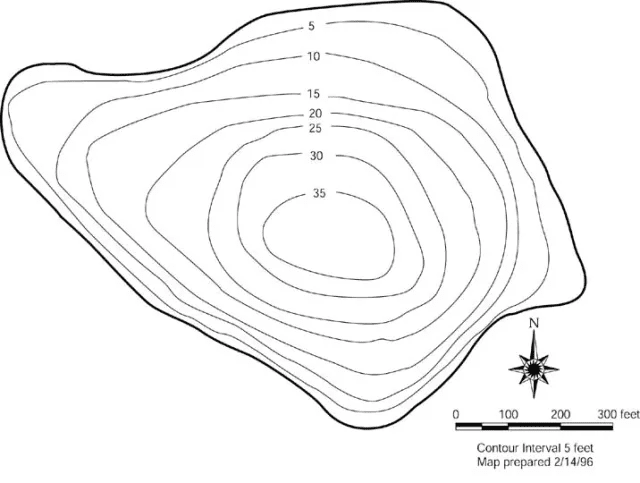
\includegraphics[width=\linewidth]{ContourMap}
				\end{center}
			\end{column}
			\begin{column}{0.5\linewidth}
				\begin{alertblock}{}\justifying\centering
					Еквіпотенціальні поверхні --- карта висот в електростатичному полі!
				\end{alertblock}
				\begin{center}
					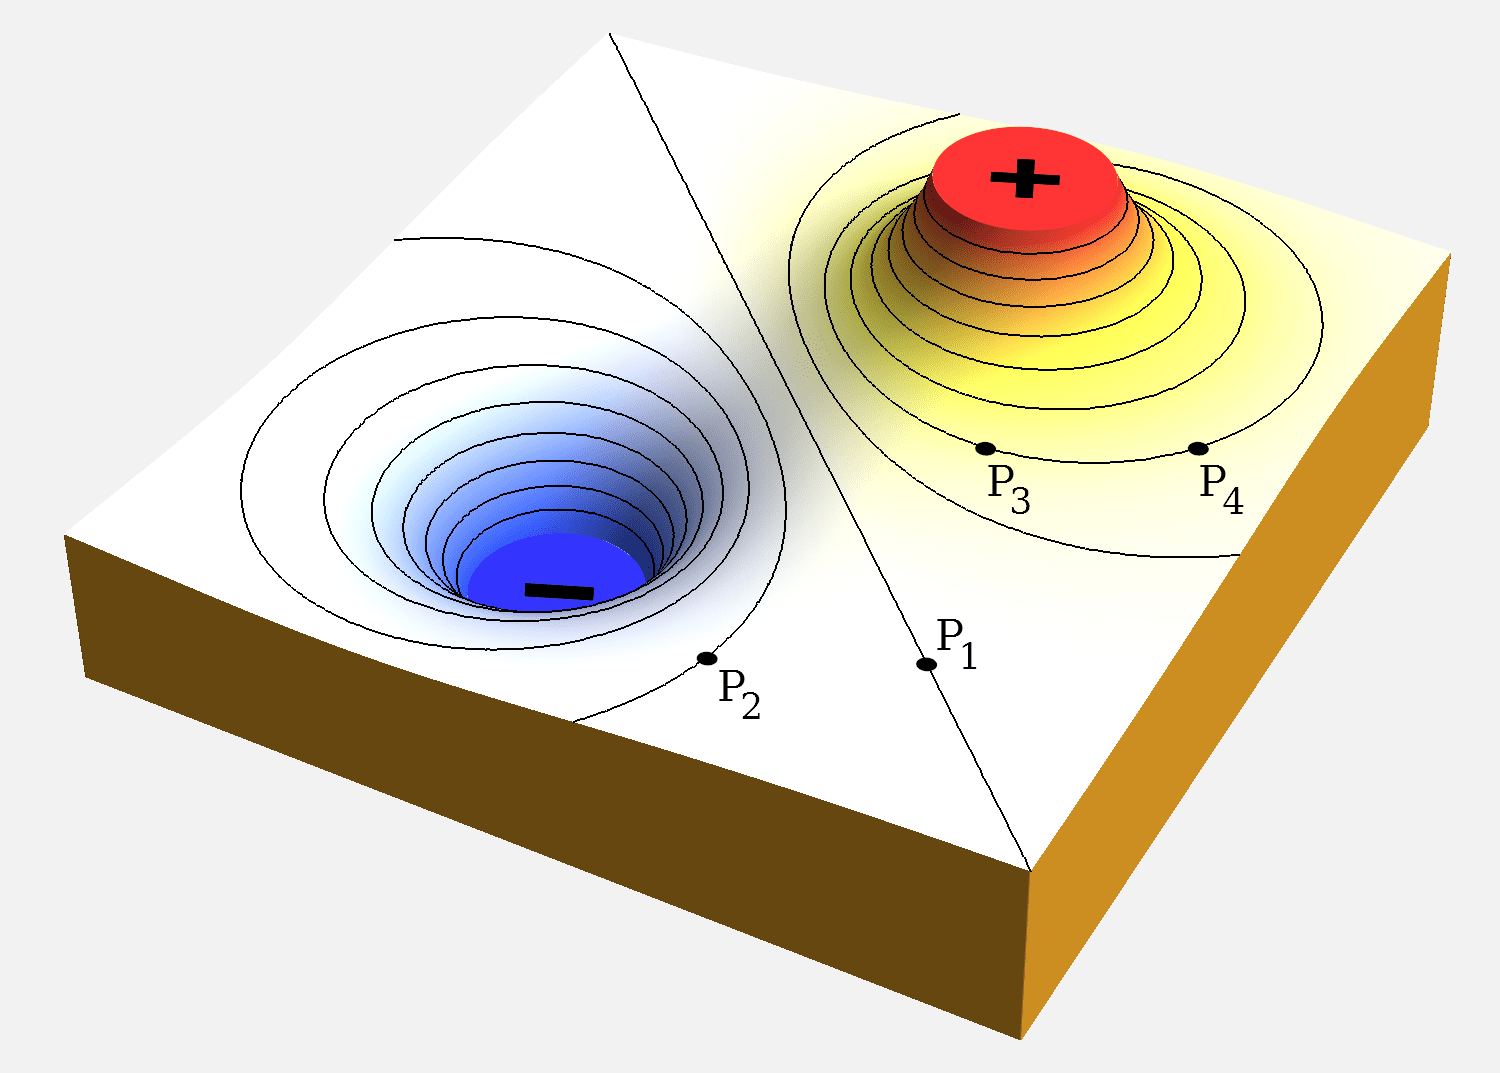
\includegraphics[width=\linewidth]{ep3d}
				\end{center}
			\end{column}
		\end{columns}
	\end{onlyenv}
	\begin{onlyenv}<3>
		\begin{center}
			\includegraphics[width=1\linewidth]{fieldlines}
		\end{center}
		\href{https://drive.google.com/file/d/1vyp5EpchboRtNrRVEHsv4h_Tsy6TSmQd/view?usp=sharing}{Побудова
			еквіпотенціальних поверхонь в Python}
	\end{onlyenv}
\end{frame}
% ===========================================================================



% ============================== Слайд ## ===============================
\begin{frame}{Властивості потенціалу}
	\begin{enumerate}\justifying
		\item Потенціал електричного поля є \alert{скалярною величиною},
		      тобто він визначається одним числом в кожній точці простору.
		\item Потенціал $\phi$ як і потенційна енергія $U$, визначається
		      \alert{з точністю до довільної константи}.

		      \begin{alertblock}{}\justifying\small
			      Значення цієї константи не відіграє ролі, оскільки фізичні явища залежать
			      тільки від напруженостей електричних полів. За нульовий потенціал зручно
			      приймати потенціал нескінченно віддаленої точки простору. На практиці за
			      нульовий потенціал зазвичай приймають потенціал Землі.
		      \end{alertblock}

		\item Потенціал підпорядковується принципу суперпозиції. Тобто, якщо
		      електричне поле створюється системою зарядів, то загальний
		      потенціал у точці $P$ є \alert{сумою
			      потенціалів}, створених кожним із цих зарядів.
		      \begin{equation*}
			      \phi = \sum_{i = 1}^{n} \phi_i.
		      \end{equation*}

		\item Потенціал електричного поля є \alert{неперервною функцією
			      простору}.

		      \begin{block}{}\justifying\small
			      Це означає, що в будь-якій точці простору (за
			      винятком  місць розташування точкових зарядів) потенціал
			      змінюється плавно і
			      не має розривів. \alert{фізичне доведення випливає із зв'язку
				      потенціалу та напруженості}.
		      \end{block}
	\end{enumerate}
\end{frame}
% ===========================================================================



% ============================== Слайд ## ===================================
\begin{frame}{Потенціал поля точкового диполя}{}
	\begin{columns}
		\begin{column}{0.7\linewidth}
			\begin{block}{}\justifying\small
				Потенціал поля точкового диполя можна знайти за допомогою принципу
				суперпозиції та з урахуванням нерівності $\ell \ll r$:
				\begin{equation*}
					\phi = \frac{(-q)}{r_-} +
					\frac{(+q)}{r_+}, \quad
					\begin{cases}
						\vec{r}_- =  \vec{r} + \vec{\ell}/2 \\
						\vec{r}_+ =  \vec{r} - \vec{\ell}/2
					\end{cases}.
				\end{equation*}
				\begin{equation*}
					\tcbhighmath{
						\phi = \frac{\vect{p}\cdot\vect{r}}{r^3}.
					}
				\end{equation*}

				Таким чином, потенціал поля точкового диполя зменшується з
				відстанню за законом
				\begin{equation*}
					\phi \sim 1/{r^2}.
				\end{equation*}
			\end{block}
		\end{column}
		\begin{column}{0.3\linewidth}
			\begin{column}{0.25\linewidth}\centering
				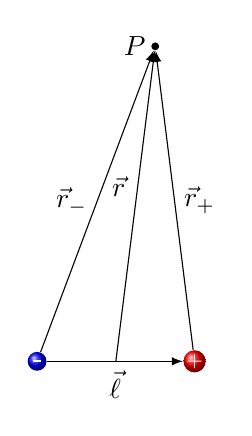
\begin{tikzpicture}[>=latex]
	\node [circle, ball color=blue, inner sep=1.2pt, text=white]
	(qn) at (-1,0) {\tikz\draw[thick] (0,0) -- ++(0.1,0);};

	\node [circle, ball color=red, inner sep=0pt, text=white,
		font=\scriptsize] (qp) at (1,0) {$+$};

	\draw[->] (qn) -- node[below] {$\vec{\ell}$} (qp);

	\node[fill, circle, inner sep=1pt] (P) at  (0.5, 4) {};
	\node[left] at (P) {$P$};

	\draw[->] (0,0) -- node[above left] {$\vec{r}$} (P);

	\draw[->] (qn) -- node[left] {$\vec{r}_-$} (P);
	\draw[->] (qp) -- node[right] {$\vec{r}_+$} (P);
\end{tikzpicture}
			\end{column}
		\end{column}
	\end{columns}
\end{frame}
% ===========================================================================



% ============================== Слайд ## ===================================
\begin{frame}{Математичні відомості}{}\small
	\begin{columns}
		\begin{column}{0.5\linewidth}
			\begin{block}{}\justifying
				Для скалярної функції однієї змінної справедливий наближений вираз:
				\begin{equation*}
					f(x + \epsilon) = f(x) + \frac{df}{dx}\epsilon, \quad \epsilon \to 0.
				\end{equation*}
			\end{block}
		\end{column}
		\begin{column}{0.5\linewidth}\centering
			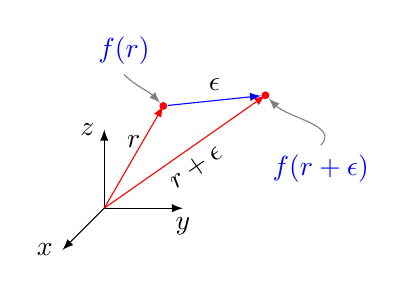
\begin{tikzpicture}[>=latex]
\draw[->] (0,0) -- ++(0, 1) node[left] {$z$};
\draw[->] (0,0) -- ++(1, 0) node[below] {$y$};
\draw[->] (0,0) -- ++(-135:0.75) node[left] {$x$};
\draw[->, red] (0,0) -- node[above, text=black] {$\vect{r}$} (60:1.5) node[inner sep=1pt,
circle,
fill] (A) {};
\draw[->, red] (0,0) -- node[below, text=black, sloped] {$\vect{r} + \vect{\epsilon}$}
(35:2.5) node[inner sep=1pt, circle, fill] (B) {};
\draw[->, blue] (A) -- node[above, text=black] {$\vect{\epsilon}$} (B);

\node[text=blue] (fr) at (0.25, 2) {$f(\vect{r})$};
\draw[gray, ->] (fr.south) to[out=-45, in=135] (A);

\node[text=blue] (fre) at (2.75, 0.5) {$f(\vect{r} + \vect{\epsilon})$};
\draw[gray, ->] (fre.north) to[out=45, in=-45] (B);

\end{tikzpicture}
		\end{column}
	\end{columns}
	\begin{block}{}\justifying

		Це співвідношення легко узагальнюється для випадку скалярної функції кількох просторових змінних:
		\begin{multline*}
			f(x + \epsilon_x, y + \epsilon_y, z + \epsilon_z) = \\
			f(x, y, z) +
			\frac{\partial f(x, y, z)}{\partial x} \epsilon_x +
			\frac{\partial f(x, y, z)}{\partial y} \epsilon_y +
			\frac{\partial f(x, y, z)}{\partial z} \epsilon_z, \quad \epsilon_x, \epsilon_y,
			\epsilon_x  \to 0.
		\end{multline*}
	\end{block}
	\begin{columns}
		\begin{column}{0.5\linewidth}
			\begin{block}{}
				\alert{Для скалярної функції} $f(\vect{r})$:
				\begin{equation*}
					\tcbhighmath{
						f(\vect{r} + \vect{\epsilon}) = f(\vect{r}) +
						\vect{\epsilon}\cdot\vect{\nabla}f(\vect{r}).
					}
				\end{equation*}
			\end{block}
		\end{column}
		\begin{column}{0.5\linewidth}
			\begin{block}{}
				\alert{Для векторної функції} $\vect{f}(\vect{r})$:
				\begin{equation*}\tcbhighmath{
						\vect{f}(\vect{r} + \vect{\epsilon}) = \vect{f}(\vect{r}) +
						(\vect{\epsilon}\cdot\vect{\nabla})\vect{f}(\vect{r}).
					}
				\end{equation*}
			\end{block}
		\end{column}
	\end{columns}

\end{frame}
% ===========================================================================

% ============================== Слайд ## ===================================
\begin{frame}{Сила, що діє на диполь в неоднорідному полі}{}
	\begin{block}{}\justifying
		Якщо \alert{диполь перебуває в неоднорідному полі} --- виникає \alert{результуюча сила}, що діє
		на диполь як  ціле, що \alert{втягуватиме диполь в область сильного поля}.
	\end{block}
	\begin{columns}
		\begin{column}{0.6\linewidth}
			\begin{block}{}\justifying
				\begin{equation*}
					\vect{F} = (+q)\Efield_+ + (-q)\Efield_- = q(\Efield_+ - \Efield_-) =
					q\Delta\Efield.
				\end{equation*}
				Для точкового диполя різницю $\Delta\Efield$ можна наближено замінити диференціалом
				\begin{equation*}
					\Delta\Efield = \Efield(\vect{r} + \vect{\ell}) - \Efield(\vect{r})= \ell_x
					\frac{\partial\Efield}{\partial x} +
					\ell_y \frac{\partial\Efield}{\partial y} + \ell_z
					\frac{\partial\Efield}{\partial z}.
				\end{equation*}
				\begin{equation*}\tcbhighmath{
						\vect{F} = p_x \frac{\partial\Efield}{\partial x} +
						p_y \frac{\partial\Efield}{\partial y} + p_z \frac{\partial\Efield}{\partial z}
						=
						(\vect{p}\cdot\vect{\nabla})\Efield.
					}
				\end{equation*}
			\end{block}
		\end{column}
		\begin{column}{0.4\linewidth}\centering
			\begin{tikzpicture}[>=latex, midarrow/.style={%
   postaction={ decorate,
   decoration={ markings, mark=at position .7 with {\arrow{latex}}}}}]

    \foreach \y in {-3,...,3}{
        \draw[red, midarrow] plot[domain=1:4] (\x, 0.2*\y+0.05*\y*\x^2);
    }

	\node [circle, ball color=blue, inner sep=1.2pt, text=white]
	(qn) at (2.5,-1) {\tikz\draw[thick] (0,0) -- ++(0.1,0);};

	\node [circle, ball color=red, inner sep=0pt, text=white,
		font=\scriptsize] (qp) at (3.3,1.45) {$+$};

        \draw[->, thick] (qp) -- ++(36:1) node[above] {$+q\Efield_+$};
        \draw[->, thick] (qn) -- ++(155:2) node[above] {$-q\Efield_-$};
        \draw[->, thick] (qn) -- (qp) node[right, pos=0.6] {$\vect{\ell}$};

\end{tikzpicture}
		\end{column}
	\end{columns}
\end{frame}
% ===========================================================================





% ============================== Слайд ## ===================================
\begin{frame}{Енергія жорсткого диполя в електричному полі}{}
	\begin{block}{}\justifying
		Енергія точкового заряду $q$ у зовнішньому полі дорівнює $U = q\phi$, де $\phi$ ---
		потенціал поля в точці знаходження заряду $q$. Диполь --- це система з двох зарядів, тому
		його енергія в зовнішньому полі
		\begin{equation*}
			U= q\phi_+ + (-q)\phi_- = q (\phi_+ - \phi_-) = q \vect{\ell}\cdot\vect{\nabla}\phi.
		\end{equation*}
		Оскільки $-\vect{\nabla}\phi = \Efield$, а $\vect{p} = q\vect{\ell}$:
		\begin{equation*}
			\tcbhighmath{
				U = -\vect{p}\cdot\Efield.
			}
		\end{equation*}
	\end{block}
	\begin{columns}
		\begin{column}{0.75\linewidth}
			\begin{block}{}\justifying\small
				Мінімальну енергію диполь має в положенні $\vect{p}
					\uparrow\uparrow \Efield$ (положення стійкої рівноваги). У разі відхилення з
				цього
				положення
				виникає момент зовнішніх сил, що повертає диполь до положення рівноваги.
			\end{block}
		\end{column}
		\begin{column}{0.25\linewidth}\centering
			\begin{tikzpicture}[>=latex, midarrow/.style={%
				postaction={ decorate,
						decoration={ markings, mark=at position .5 with {\arrow{latex}}}}}]

	\foreach \y in {-2,...,2}{
			\draw[red, midarrow] plot[domain=1:4] (\x, 0.2*\y);
		}

	\node [circle, ball color=blue, inner sep=1.2pt, text=white]
	(qn) at (2,0) {\tikz\draw[thick] (0,0) -- ++(0.1,0);};

	\node [circle, ball color=red, inner sep=0pt, text=white,
		font=\scriptsize] (qp) at (3,0) {$+$};


	\draw[->, thick] (qn) --  node[below, circle, inner sep=1pt, fill=white]
	{$\vect{p}$} (qp);

    \begin{scope}[yshift=-1.5cm]
             				\foreach \y in {-2,...,2}{
			\draw[red, midarrow] plot[domain=1:4] (\x, 0.2*\y);
		}

	\node [circle, ball color=blue, inner sep=1.2pt, text=white]
	(qn) at (2,0.25) {\tikz\draw[thick] (0,0) -- ++(0.1,0);};

	\node [circle, ball color=red, inner sep=0pt, text=white,
		font=\scriptsize] (qp) at (3,-0.25) {$+$};

	\draw[->, thick] (qn) --  node[anchor=north east, circle, inner sep=1pt,
	fill=white]
	{$\vect{p}$} (qp);
    \end{scope}
\end{tikzpicture}
		\end{column}
	\end{columns}
\end{frame}
% ===========================================================================




% ============================== Слайд ## ===================================
\begin{frame}{Енергія пружного диполя в електричному полі}{}
	\begin{block}{}\justifying
		Під дією електричного поля плече диполя збільшується на таку величину $\ell$, що сила з боку
		поля врівноважується силою пружності
		$
			k\ell = qE
		$.
		Звідси знаходимо, що дипольний момент $p = q\ell$ залежить від прикладеного поля за законом:
		\begin{equation*}
			p = \frac{q^2E}{k} = \alpha E
		\end{equation*}
		Коефіцієнт $\alpha$ називається \alert{поляризованістю молекули}.

		\smallskip

		Потенціальна енергія деформації дорівнює
		$
			U = \frac{k\ell^2}2
		$.
		Оскільки $k = \frac{qE}{\ell}$, одержимо
		$
			U = \frac{k\ell^2}2 = \frac{q\ell E}2 = \frac{pE}2
		$.
		Тут вектор дипольного моменту, індукований зовнішнім полем, паралельний електричному полю
		$\vect{p}\uparrow\uparrow \Efield$. Тому останню формулу можна переписати у векторній формі:
	\end{block}
	\begin{equation*}
		\tcbhighmath{
			U = \frac12\ \vect{p}\cdot\Efield.
		}
	\end{equation*}
\end{frame}
% ===========================================================================



% ===========================================================================
\begin{frame}{Рівняння Пуассона та Лапласа}
	\begin{block}{}\small
		Оскільки $\Efield = - \vect{\nabla}\phi$ , $\divg\Efield  = 4\pi\rho$, то
		звідси випливає \alert{рівняння Пуассона для потенціалу поля}:
		\begin{equation*}
			\tcbhighmath{
				\nabla^2\phi = - 4\pi\rho.
			}
		\end{equation*}
	\end{block}
	\begin{block}{}\small
		Тут введено оператор Лапласа (лапласіан)
		$
			\nabla^2 = \frac{\partial^2}{\partial x^2} +
			\frac{\partial^2}{\partial y^2} + \frac{\partial^2}{\partial z^2}
		$.
	\end{block}
	\begin{block}{}
		У області простору, вільній від зарядів ($\rho = 0$ ), рівняння Пуассона
		зводиться до \alert{рівняння Лапласа}
		\begin{equation*}
			\tcbhighmath{
				\nabla^2\phi = 0 .
			}
		\end{equation*}
	\end{block}

	\begin{block}{}\justifying\small
		Загальна електростатична задача зводиться до знаходження розв'язку
		рівняння Пуассона (або Лапласа).

		\medskip

		Ця задача має \alert{єдиний розв'язок}. Якщо розв'язок не один, то буде не один електричний
		<<ландшафт>>, отже, у кожній точці поле $\Efield$, узагалі кажучи, неоднозначне --- що є
		фізичного абсурдним. Це твердження називають \alert{теоремою єдиності}.
	\end{block}
\end{frame}
% ===========================================================================





% ============================== Слайд ## ===================================
\begin{frame}{Граничні умови}{}
	\begin{block}{}
		При переході через границю розділу середовищ електричне поле змінюється за
		певними законами.
	\end{block}
	\begin{onlyenv}<1>
		\begin{columns}
			\begin{column}{0.6\linewidth}
				\begin{block}{}\small\justifying
					Застосуємо теорему Гаусса до нескінченно малого циліндра, що охоплює частину межі
					розділу двох
					середовищ. Вважаючи $d\vect{S}_1 = - d\vect{S}_2$, $q = \sigma dS$,
					$d\vect{S}_1 =
						\vect{n}\ dS$,
					маємо
				\end{block}
			\end{column}
			\begin{column}{0.4\linewidth}\centering
				 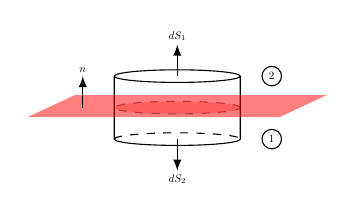
\begin{tikzpicture}[
scale=0.4,
transform shape,
>=latex,
declare function = {
h = 2;
r=2;
r2=0.2;
},
]

\fill[red!50, opacity=0.5, draw=black, dashed] (0,1) circle (r and r2);
\draw (-2,h) -- (-2,0) arc (180:360:r and r2) -- (2,h) ++ (-2,0) circle (r and r2);
\draw[dashed] (-2,0) arc (180:0:r and r2);
\fill[red,opacity=0.5]
 (-4.75,0.7) -- ++(8,0) -- ++(1.5,0.7) -- ++(-8,0) ;
\draw[->] (0,h) -- ++(0,1) node[above] {$d\vect{S}_1$};
\draw[->] (0,0) -- ++(0,-1) node[below] {$d\vect{S}_2$};

\draw[->] (-3,1) -- ++(0,1) node[above] {$\vect{n}$};

\node[circle, draw] at (3,0) {$1$};
\node[circle, draw] at (3,h) {$2$};
\end{tikzpicture}
			\end{column}
		\end{columns}
		\begin{block}{}\small
			\begin{equation*}
				\oiint_S \Efield\cdot d\vect{S} = 4\pi\sigma\ \Rightarrow  \Efield\cdot
				d\vect{S}_1 +
				\Efield\cdot d\vect{S}_2 = 4\pi\sigma dS
			\end{equation*}
		\end{block}
		\begin{block}{}
			Звідси випливає перша гранична умова:
			\begin{equation*}
				\tcbhighmath{
					E_{1n} - E_{2n} = 4\pi\sigma.
				}
			\end{equation*}
		\end{block}
		\begin{alertblock}{}\justifying\small
			Нормальна складова вектора $\Efield$ зазнає стрибка при
			переході через заряджену границю розділу. Однак якщо заряди на межі розділу відсутні
			($\sigma =
				0$), то $E_{1n} = E_{2n}$ і стрибка не буде.
		\end{alertblock}
	\end{onlyenv}
	\begin{onlyenv}<2>
		\begin{columns}
			\begin{column}{0.6\linewidth}
				\begin{block}{}\small\justifying
					Застосуємо теорему про циркуляцію до нескінченно малого прямокутного
					контуру $L$, що проходить на нескінченно малій відстані над і під поверхнею
					розділу середовищ. Вважаючи, що $d\vect{r}_1 = -d\vect{r}_2$, маємо
				\end{block}
			\end{column}
			\begin{column}{0.4\linewidth}\centering
				 \begin{tikzpicture}[
scale=0.4,
transform shape,
>=latex,
declare function = {
h = 2;
r=2;
r2=0.2;
},
midarrow/.style={%
   postaction={ decorate,transform shape,
   decoration={ markings, mark=at position .5 with {\arrow{>}}}}},
]

\fill[red,opacity=0.5]
 (-4.75,0.7) -- ++(8,0) -- ++(1.5,0.7) -- ++(-8,0) ;

\draw[midarrow] (2, 1) -- ++(0, 1) -- node[above=5pt] {$L$} ++(-4, 0) -- ++(0, -1);
\draw[midarrow] (-2, 1) -- ++(0, -1) -- ++(4, 0) -- ++(0, 1);

\draw[->] (-3,1) -- ++(-2,0) node[above] {$\vect{\tau}$};
\draw[->] (-3,1) -- ++(0,1) node[above] {$\vect{n}$};
\draw[->] (-3,1) -- ++({180+45}:1) node[below] {$\vect{b}$};
\node[circle, draw] at (3,0) {$1$};
\node[circle, draw] at (3,h) {$2$};
\end{tikzpicture}
			\end{column}
		\end{columns}
		\begin{block}{}\small
			\begin{equation*}
				\oint\limits_L \Efield\cdot d\vect{r} = 0 \Rightarrow \Efield_1 d\vect{r}_1 +
				\Efield_2 d\vect{r}_2 = 0
			\end{equation*}
		\end{block}
		\begin{block}{}
			Звідси випливає друга гранична умова:
			\begin{equation*}
				\tcbhighmath{
					E_{1\tau} = E_{2\tau}.
				}
			\end{equation*}
		\end{block}
		\begin{alertblock}{}\justifying\small
			Тангенціальна складова $\Efield$ виявляється однаковою по обидва боки границі розділу (не
			зазнає стрибка).
		\end{alertblock}
	\end{onlyenv}
\end{frame}
% ===========================================================================



% ============================== Слайд ## ===================================
\begin{frame}{Задачі}{}
	\begin{exampleblock}{Задача}\justifying
		Використовуючи теорему Гаусса в диференціальній формі знайдіть напруженість
		електричного поля всередині та зовні однорідно зарядженої кулі. Заряд кулі дорівнює
		$Q$, радіус кулі~$R$.
	\end{exampleblock}
\end{frame}
% ===========================================================================



% ============================== Слайд ## ===================================
\begin{frame}{Підсумки}{}
	\framesubtitle<1>{Означення}
	\framesubtitle<2>{Основні рівняння та теореми}
	\framesubtitle<3>{Поля та сили}
	\begin{overprint}
		\onslide<1>
		\begin{tblr}{QQ[mode=math]}
			Напруженість поля & \Efield = \frac{\vect{F}}{q}          \\
			Потенціал поля    & \phi = \frac{U}{q}                    \\
			Потік поля        & \iint\limits_S \Efield\cdot d\vect{S} \\
			Циркуляція поля   & \oint\limits_L \Efield\cdot d\vect{r}
		\end{tblr}
		\onslide<2>
		\begin{tblr}{QQ[mode=math]}
			Теорема Гаусса в інтегральній формі      & \oiint\limits_S
			\vec{E}\cdot
			d\vec{S} = 4\pi \iiint\limits_V \rho
			dV                                                                       \\
			Теорема про циркуляцію вектора $\Efield$ & \oint\limits_L \Efield\cdot
			d\vect{r} = 0
			\\
			Теорема Гаусса в диференціальній формі   & \divg\Efield =
			4\pi\rho.
			\\
			Вихор електростатичного поля             & \rot\Efield =
			0
			\\
			Зв'язок напруженості та потенціалу       & \Efield = - \vect{\nabla}\phi \\
			Рівняння Пуассона                        & \nabla^2\phi = -4\pi\rho      \\
			Рівняння Лапласа                         & \nabla^2\phi = 0              \\
			Граничні умови                           & E_{1n} - E_{2n} = 4\pi\sigma  \\
			                                         & E_{1\tau} = E_{2\tau}
		\end{tblr}
		\onslide<3>
		\begin{tblr}{QQ[mode=math]}
			Поле точкового заряду                        & \vec{E} = \frac{q}{r^2}\ \frac{\vec{r}}{r}            \\
			Потенціал поля точкового заряду              & \phi = \frac{q}{r}                                    \\
			Сила, що діє на точковий заряд               & \vect{F} = q\Efield                                   \\
			Енергія точкового заряду                     & U = q\phi                                             \\
			Поле, що створюється диполем                 & \vec{E} = \frac{3(\vec{p}\cdot\vec{r})\vec{r}}{r^5} -
			\frac{\vec{p}}{r^3}                                                                                  \\
			Потенціал поля диполя                        & \phi = \frac{\vect{p}\cdot\vect{r}}{r^3}              \\
			Момент, що діє на диполь                     & \vect{M} = \left[\vect{p}\times\Efield\right]         \\
			Сила, що діє на диполь                       & \vect{F} =
			(\vect{p}\cdot\vect{\nabla})\Efield.                                                                 \\
			Енергія жорсткого диполя в електричному полі & U = -\vect{p}\cdot\Efield                             \\
			Енергія пружного диполя в електричному полі  & U = \frac12\ \vect{p}\cdot\Efield                     \\
		\end{tblr}
	\end{overprint}
\end{frame}
% ===========================================================================



\end{document}
